\begingroup\sloppy
\section{Návrh doménového modelu}\label{sec:a5}

Tento artefakt popisuje implementační model aplikace tak, jak je naprogramovaný. Vychází z modelu domény v \odkaz{sec:tech}{technické specifikaci} a rozšiřuje ho o datové typy, metody, služby a rozhraní datové vrstvy. Aplikace má tři vrstvy. Prezentační vrstva (\texttt{presentation.desktop} a \texttt{presentation.web}) volá jen služby aplikační vrstvy. Aplikační vrstva (\texttt{business}) obsahuje doménový model, služby a rozhraní pro přístup k datům. Datová vrstva (\texttt{data}) tato rozhraní implementuje. Všechny části skládá dohromady třída \texttt{AppContext} při startu aplikace.

\subsection{Statický diagram tříd aplikační vrstvy}\label{sec:a5:bl}

Statický diagram tříd je kvůli čitelnosti rozdělený do šesti obrázků podle balíčků. Atributy jsou privátní (\texttt{-}) a mají implementační datové typy. Metody jsou veřejné obchodní operace (\texttt{+}) s parametry a návratovými typy. Gettery, settery, konstruktory a metody, které používá jen mapper při načítání (\texttt{loadCategory}, \texttt{loadItem}), v diagramech nejsou. Vazba na jiný objekt je nakreslená jako asociace s násobností a směrem navigace, a proto se už neopakuje mezi atributy. Plný kosočtverec označuje kompozici a prázdný kosočtverec agregaci. Podtržené metody jsou statické. Třída \texttt{DomainObject} je kvůli přehlednosti nakreslená ve více obrázcích.

Na rozdíl od modelu domény se některé třídy neodkazují na jiný objekt, ale jen na jeho identifikátor. Revize menu, komentář i sdílený odkaz mají atribut \texttt{menuId}. Projekt má \texttt{responsibleUserId}. Menu tedy nemá seznam revizí a revize se načítají přes \texttt{MenuService} podle čísla menu. Tento postup je jednodušší a odpovídá tomu, že se revize otevírají jednotlivě.

\clearpage
\begin{figure}[H]
  \centering
  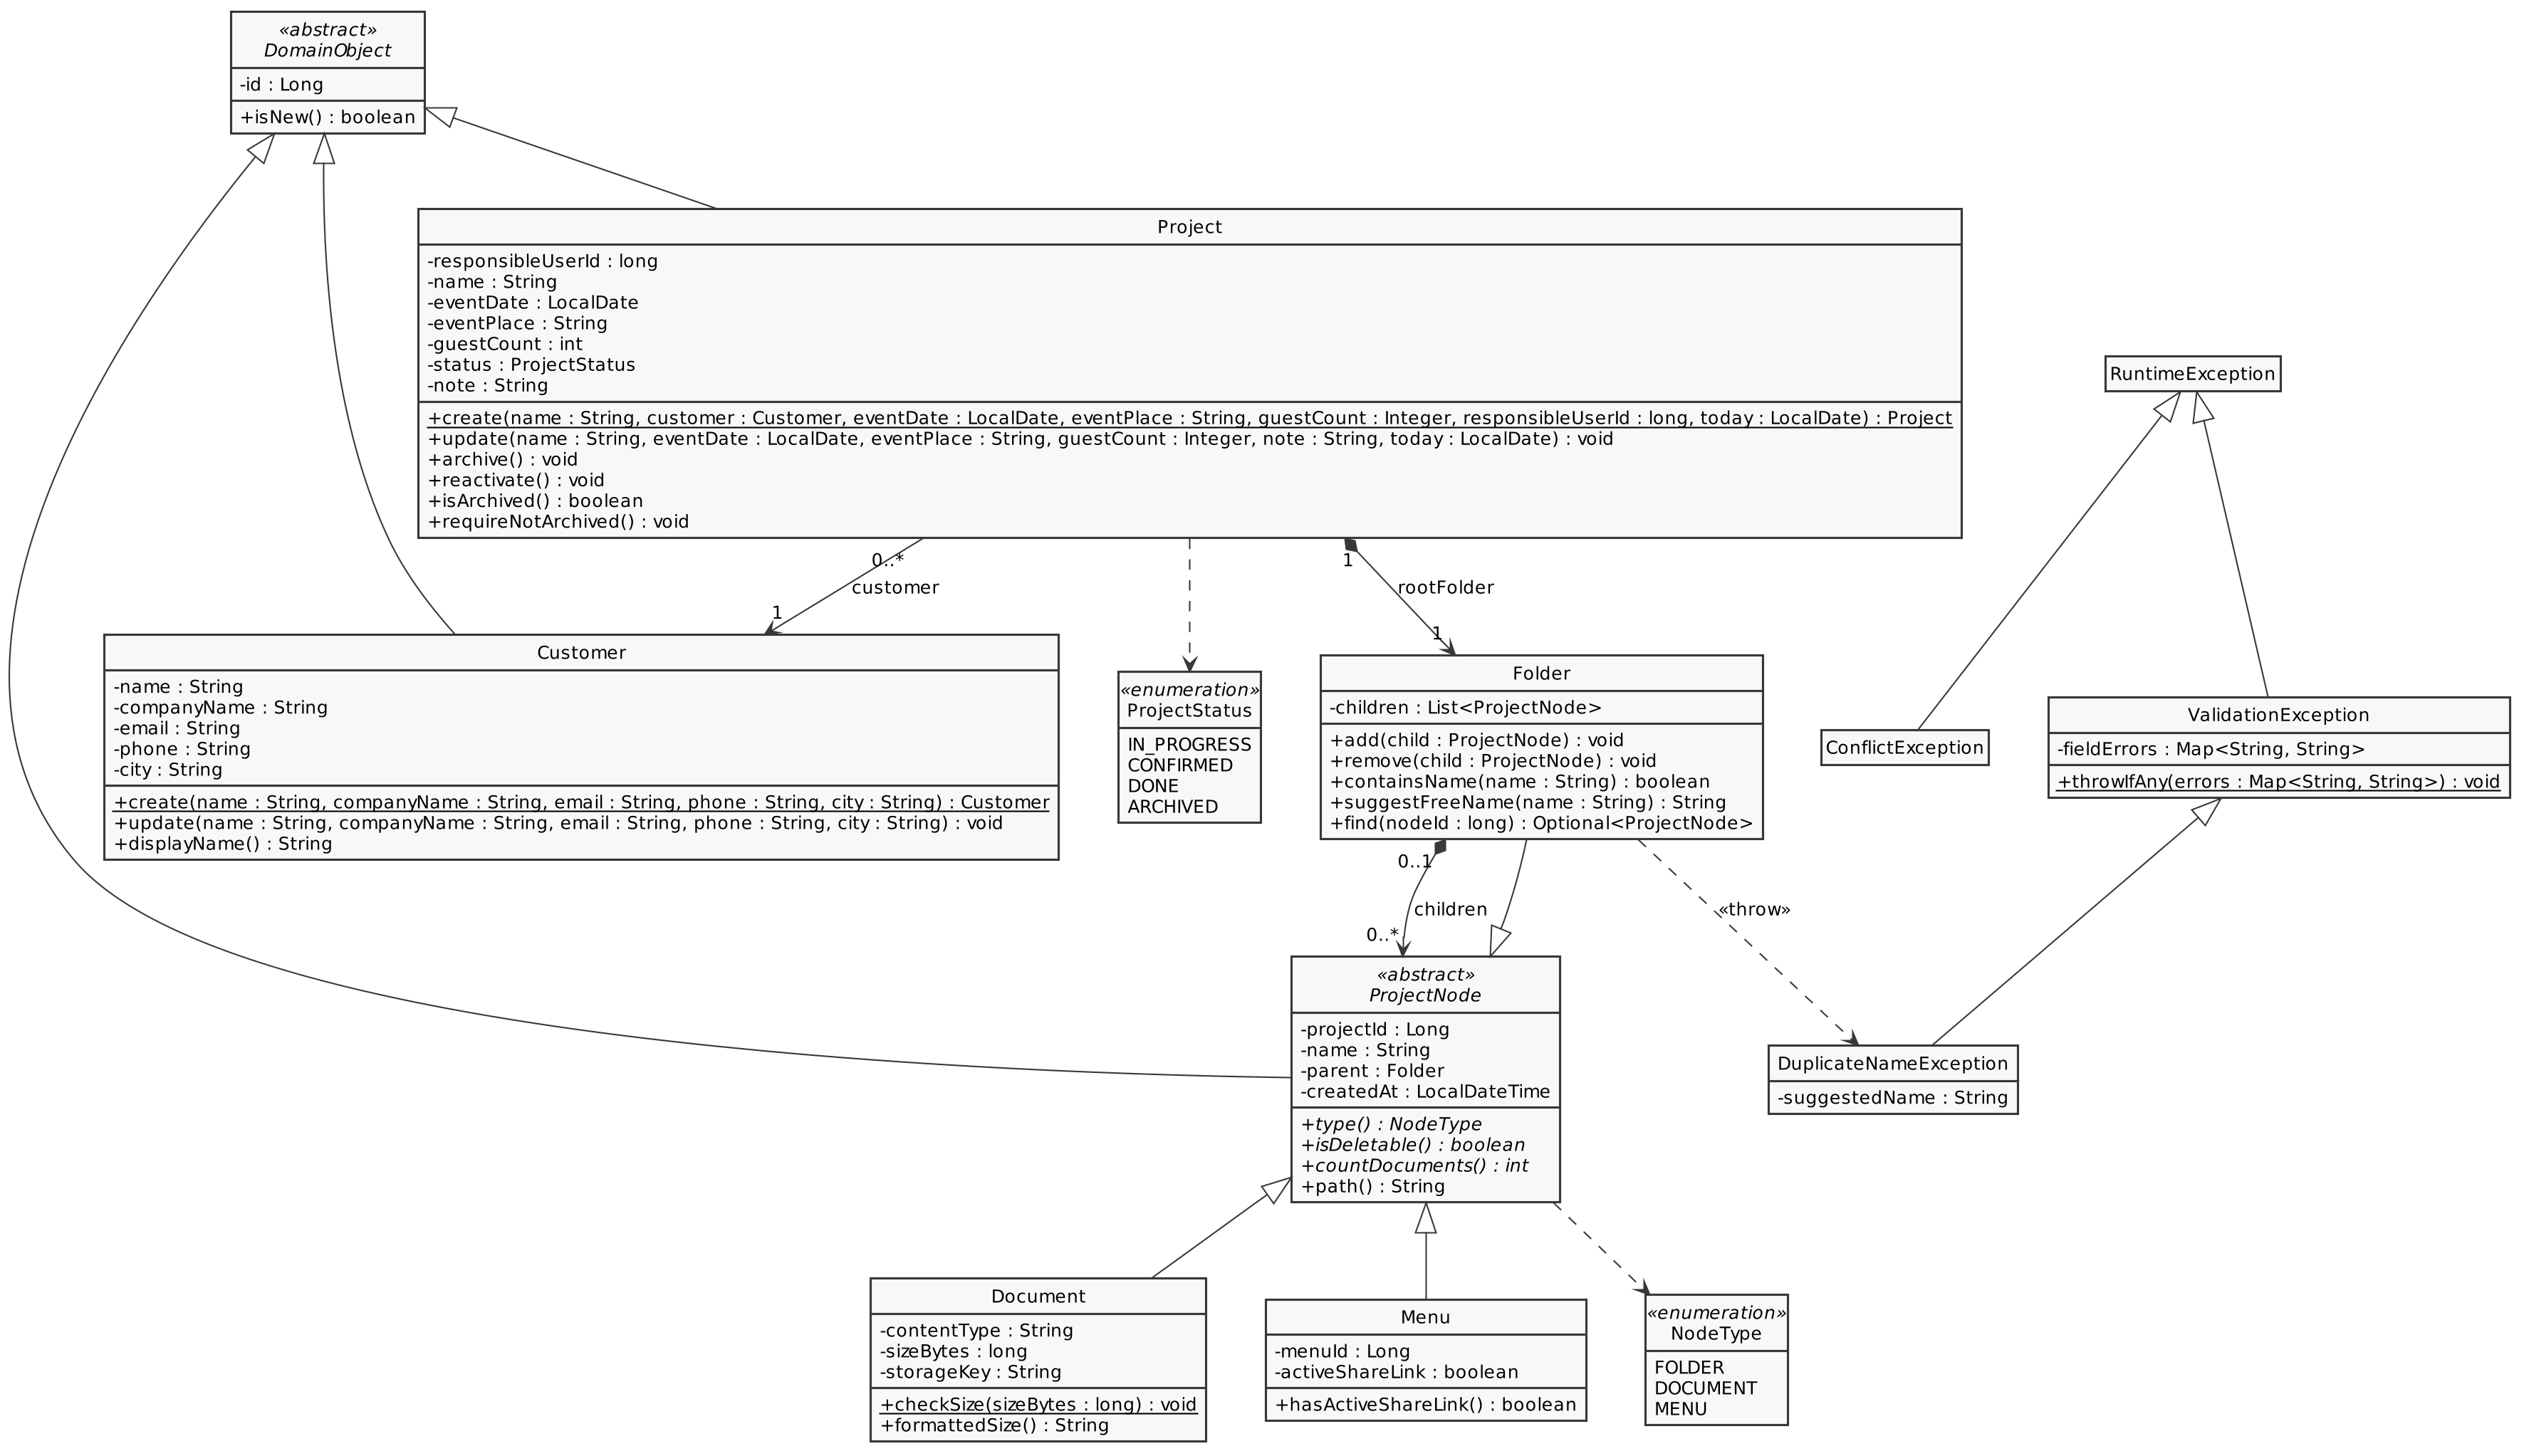
\includegraphics[width=0.85\textheight,height=\textwidth,keepaspectratio,angle=90]{class-domain-project.png}
  \caption{Diagram tříd -- projekt, zákazník a strom složek}
  \label{fig:a5:project}
\end{figure}
\clearpage

\subsubsection*{Doménový model -- projekt a strom složek (\texttt{business.domain})}

Obrázek \odkaz{fig:a5:project}{diagram tříd projektu} ukazuje projekt, zákazníka a strom složek a dokumentů z \ucref{02}.

\begin{description}[itemsep=2pt,style=unboxed]
  \item[\texttt{DomainObject}] Abstraktní předek všech entit, které mají vlastní řádek v databázi. Drží identifikátor \texttt{id} a metodou \texttt{isNew} říká, zda už byl objekt uložen.
  \item[\texttt{Customer}] Zákazník cateringu. Metody \texttt{create} a \texttt{update} kontrolují povinné údaje, formát e-mailu a telefonu.
  \item[\texttt{Project}] Zakázka pro jednu akci zákazníka. Při vytvoření ověří údaje formuláře a založí kořenovou složku. Hlídá, že archivovaný projekt už nelze měnit (\texttt{requireNotArchived}). Metoda \texttt{reactivate} vrátí archivovaný projekt do stavu rozpracovaný a jinak odmítne.
  \item[\texttt{ProjectNode}] Abstraktní uzel stromu projektu. Určuje společné operace všech uzlů, tedy typ, cestu, možnost smazání a počet dokumentů.
  \item[\texttt{Folder}] Složka, která obsahuje další uzly. Při přidání uzlu odmítne duplicitní název a nabídne volný název (\texttt{suggestFreeName}).
  \item[\texttt{Document}] Nahraný soubor. Drží typ obsahu, velikost a klíč, pod kterým je soubor uložený v úložišti dokumentů. Kontroluje limit velikosti 20~MB.
  \item[\texttt{Menu}] Uzel stromu, který představuje menu. Menu s aktivním sdíleným odkazem nelze smazat.
  \item[\texttt{ProjectStatus}] Výčet stavů projektu.
  \item[\texttt{NodeType}] Výčet typů uzlů. Jeho hodnota se ukládá jako rozlišovací sloupec v databázi.
  \item[\texttt{ValidationException}] Výjimka pro chybná vstupní data. Nese chyby jednotlivých polí formuláře, aby je uživatelské rozhraní mohlo zobrazit u správného pole.
  \item[\texttt{DuplicateNameException}] Chyba duplicitního názvu ve složce. Nese navržený volný název.
  \item[\texttt{ConflictException}] Chyba souběžné změny. Vzniká, když jiný uživatel mezitím uložil nebo sdílel stejné menu a když databáze odmítne vložení kvůli porušení jedinečnosti (\texttt{Jdbc}).
\end{description}

\clearpage
\begin{figure}[H]
  \centering
  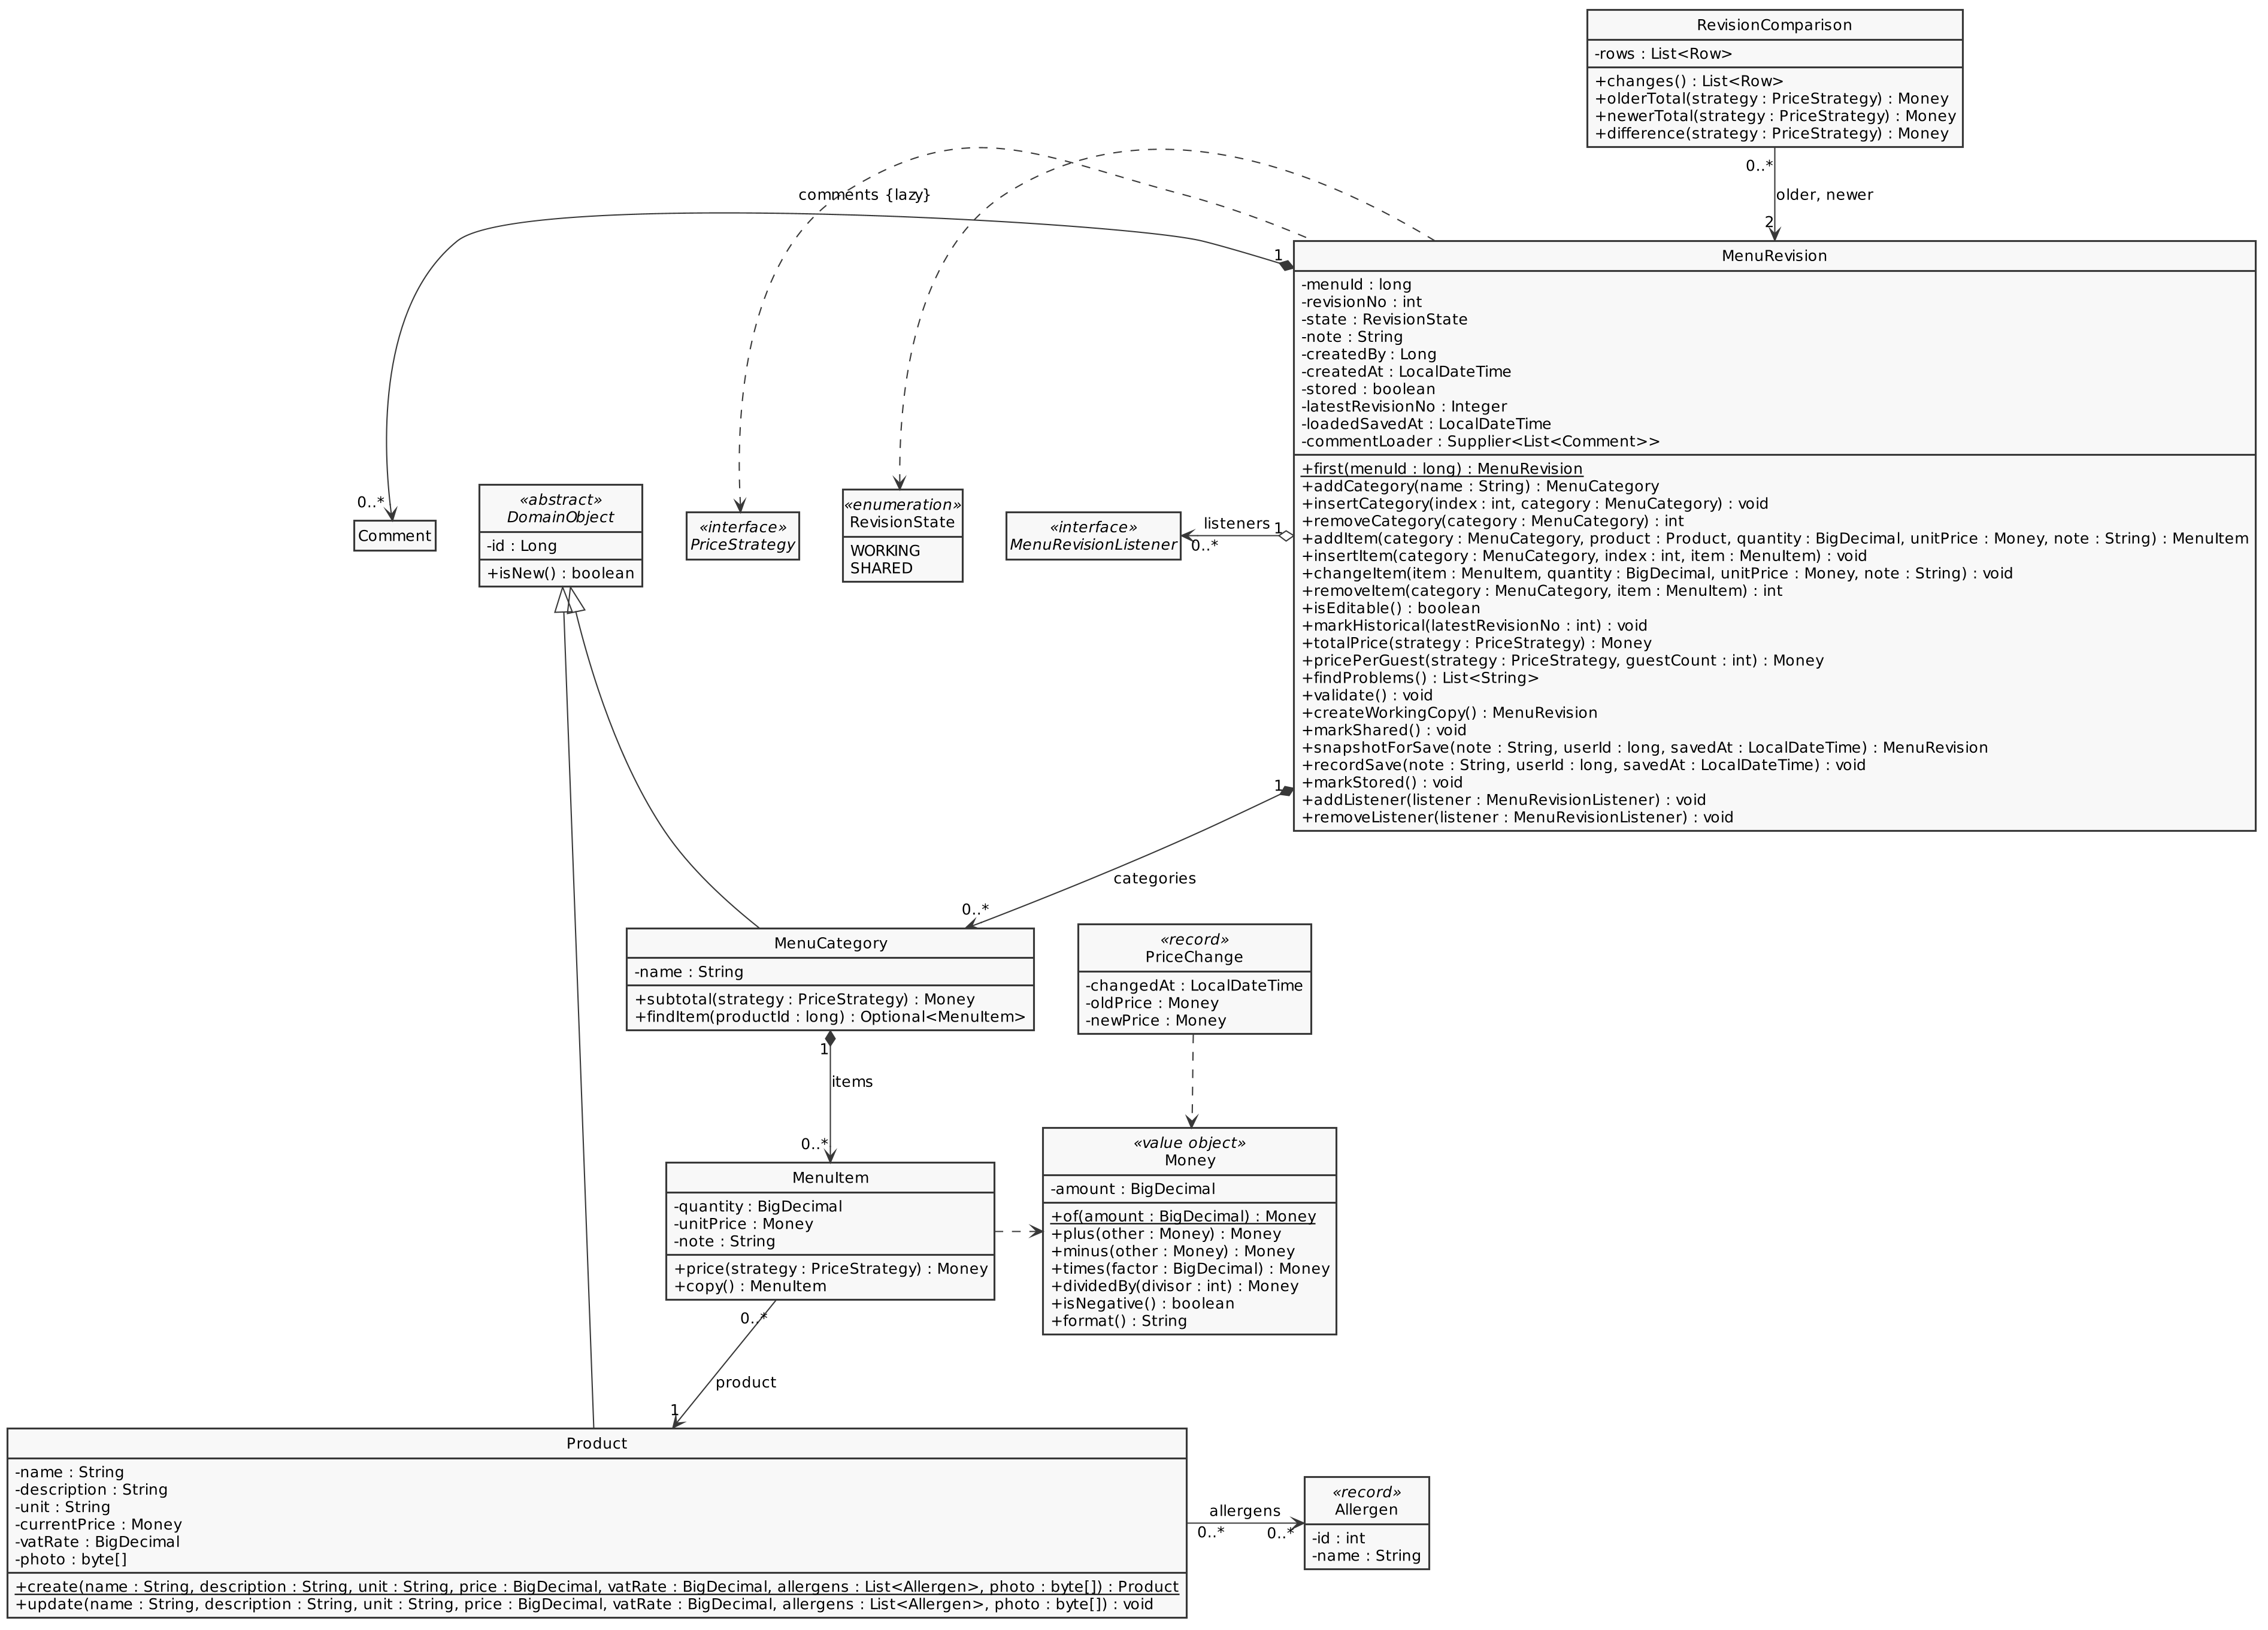
\includegraphics[width=0.85\textheight,height=\textwidth,keepaspectratio,angle=90]{class-domain-menu.png}
  \caption{Diagram tříd -- menu, revize a katalog produktů}
  \label{fig:a5:menu}
\end{figure}
\clearpage

\subsubsection*{Doménový model -- menu a katalog (\texttt{business.domain})}

Obrázek \odkaz{fig:a5:menu}{diagram tříd menu} ukazuje obsah menu z \ucref{08} a katalog produktů.

\begin{description}[itemsep=2pt,style=unboxed]
  \item[\texttt{MenuRevision}] Jedna revize menu a hlavní třída úpravy menu. Pracovní revizi lze přímo upravovat, sdílenou ani starší revizi nikoli a změny jdou do pracovní kopie s dalším číslem. Kontroluje pravidla menu (\texttt{findProblems}, \texttt{validate}), mezi která patří limity názvu kategorie (60 znaků), poznámky k položce (200 znaků), množství (nejvýše dvě desetinná místa a méně než 1~000~000) a jednotkové ceny (méně než 100~000~000), a odmítá chybějící množství nebo cenu. Metoda \texttt{snapshotForSave} vytvoří kopii hlavičky revize s údaji o uložení, kterou mapper zapíše. Samotná revize se mění až po úspěšném commitu (\texttt{recordSave}, \texttt{markStored}, u sdílení \texttt{markShared}), počítá cenu celkem a na hosta a oznamuje každou změnu posluchačům. Komentáře načítá až při prvním použití.
  \item[\texttt{MenuCategory}] Kategorie menu, například předkrmy. Obsahuje položky a počítá jejich mezisoučet.
  \item[\texttt{MenuItem}] Položka menu. Odkazuje na produkt z katalogu a drží množství, jednotkovou cenu a poznámku. Cenu řádku počítá podle zvolené cenové strategie.
  \item[\texttt{Product}] Produkt z katalogu se jménem, jednotkou, aktuální cenou, sazbou DPH, alergeny a fotografií. Metody \texttt{create} a \texttt{update} kontrolují povolené jednotky, sazby DPH, velikost fotografie a cenu (nejvýše dvě desetinná místa, méně než 100~000~000).
  \item[\texttt{Allergen}] Alergen podle číselníku (záznam s číslem a názvem).
  \item[\texttt{PriceChange}] Jeden záznam historie ceny produktu (kdy, stará a nová cena).
  \item[\texttt{Money}] Neměnná peněžní částka v Kč. Sčítá, odečítá, násobí, dělí a formátuje částky, takže se s cenou nepracuje jako s holým číslem.
  \item[\texttt{RevisionComparison}] Porovnání dvou revizí téhož menu. Vytvoří řádky přidaných, odebraných a změněných položek a rozdíl ceny.
  \item[\texttt{RevisionState}] Výčet stavů revize (pracovní a sdílená).
\end{description}

Rozhraní \texttt{PriceStrategy} a \texttt{MenuRevisionListener} jsou podrobně v \odkaz{fig:a5:gof}{diagramu vzorů GoF}. Třída \texttt{Comment} je podrobně v \odkaz{fig:a5:users}{diagramu uživatelů a sdílení}.

\clearpage
\begin{figure}[H]
  \centering
  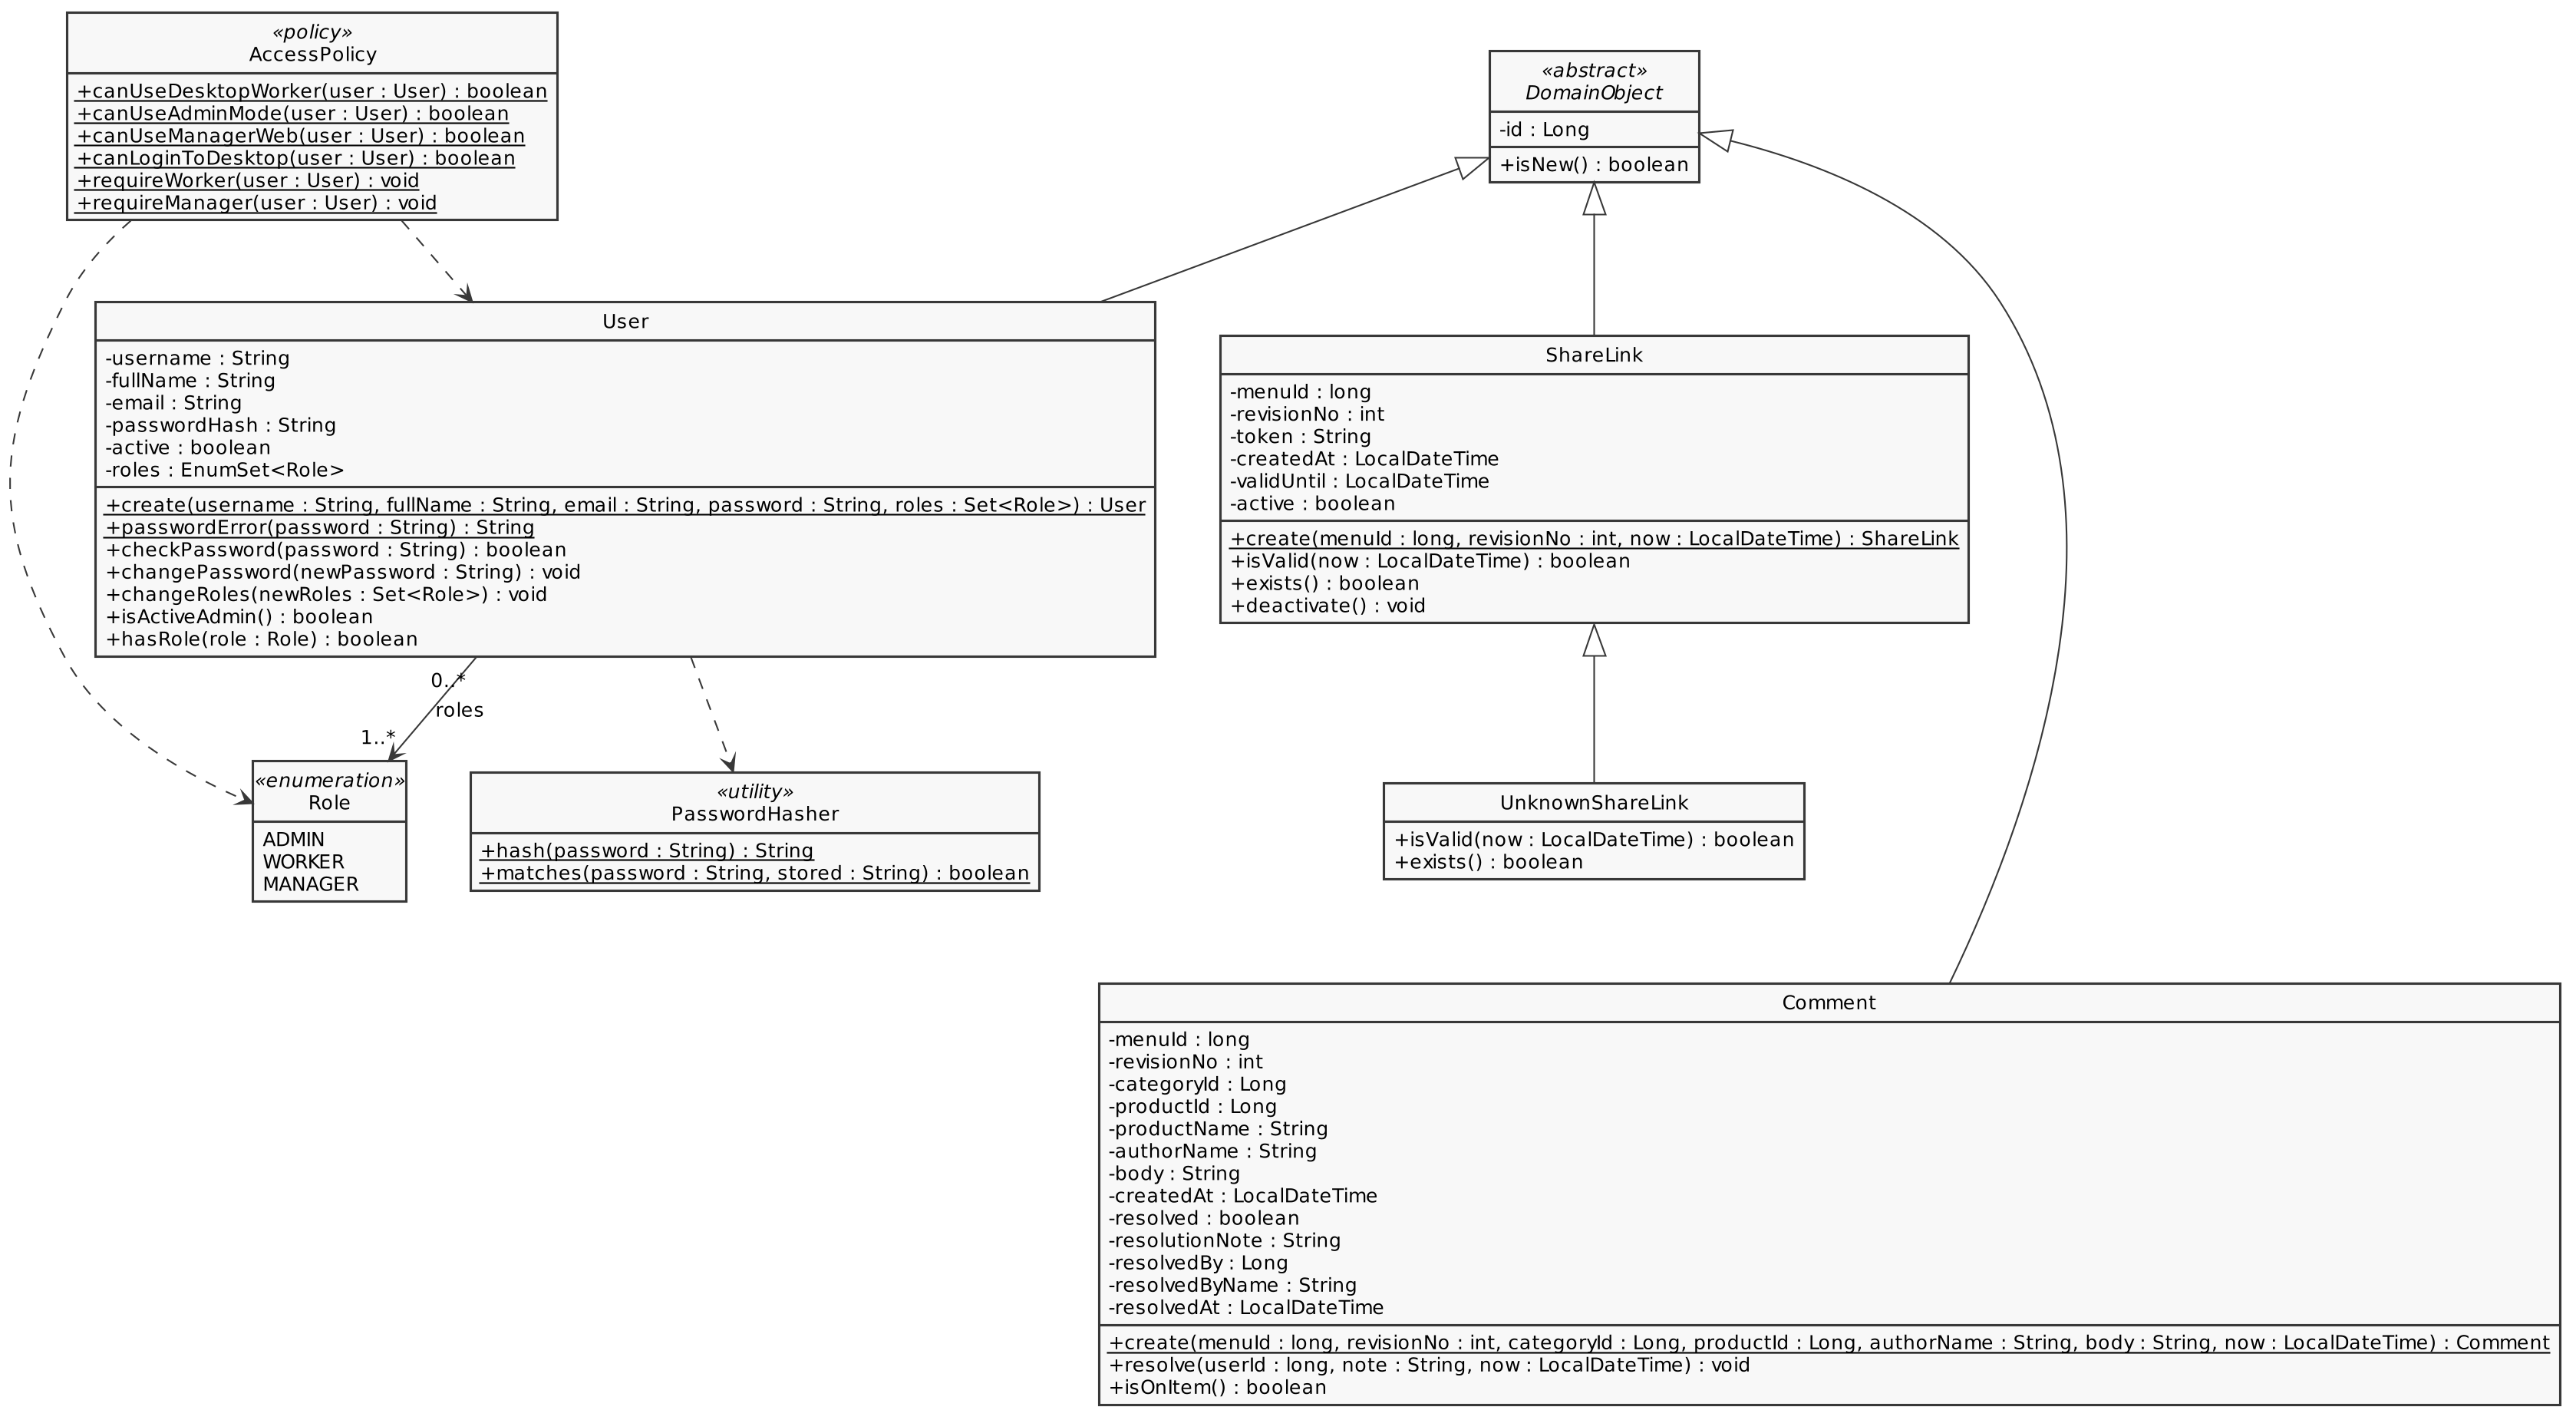
\includegraphics[width=0.85\textheight,height=\textwidth,keepaspectratio,angle=90]{class-domain-users.png}
  \caption{Diagram tříd -- uživatelé, sdílené odkazy a komentáře}
  \label{fig:a5:users}
\end{figure}
\clearpage

\subsubsection*{Doménový model -- uživatelé a sdílení (\texttt{business.domain})}

Obrázek \odkaz{fig:a5:users}{diagram tříd uživatelů a sdílení} ukazuje třídy pro \ucref{11}, \ucref{13} a \ucref{16}.

\begin{description}[itemsep=2pt,style=unboxed]
  \item[\texttt{User}] Uživatelský účet s rolemi. Při založení kontroluje údaje (celé jméno nejvýše 100 a e-mail nejvýše 254 znaků) a délku hesla, heslo ukládá jen jako otisk. Umí ověřit heslo, změnit heslo a role a zjistit, zda je uživatel aktivní administrátor.
  \item[\texttt{Role}] Výčet rolí uživatele (administrátor, pracovník, manažer).
  \item[\texttt{AccessPolicy}] Třída bez stavu, ve které jsou na jednom místě pravidla, která role co smí. Role se sčítají a každá odemyká jen svou oblast. Metody \texttt{canUseDesktopWorker}, \texttt{canUseAdminMode} a \texttt{canUseManagerWeb} vracejí, zda je aktivní uživatel pracovník, administrátor nebo manažer. Metoda \texttt{canLoginToDesktop} platí pro pracovníka nebo administrátora. Metody \texttt{requireWorker} a \texttt{requireManager} vyhodí \texttt{ValidationException}, když uživatel roli nemá.
  \item[\texttt{PasswordHasher}] Pomocná třída, která počítá a ověřuje otisk hesla algoritmem PBKDF2 se solí.
  \item[\texttt{ShareLink}] Odkaz, přes který zákazník vidí sdílenou revizi menu. Vytváří náhodný token, platí 14 dní a lze ho zneplatnit.
  \item[\texttt{UnknownShareLink}] Zvláštní případ odkazu pro token, který v databázi není. Není platný a metoda \texttt{exists} vrací \texttt{false}, takže služba nemusí řešit hodnotu \texttt{null}.
  \item[\texttt{Comment}] Komentář zákazníka k celému menu nebo k jedné položce. Kontroluje jméno autora a délku textu. Pracovník ho vyřídí metodou \texttt{resolve} s poznámkou.
\end{description}

\clearpage
\begin{figure}[H]
  \centering
  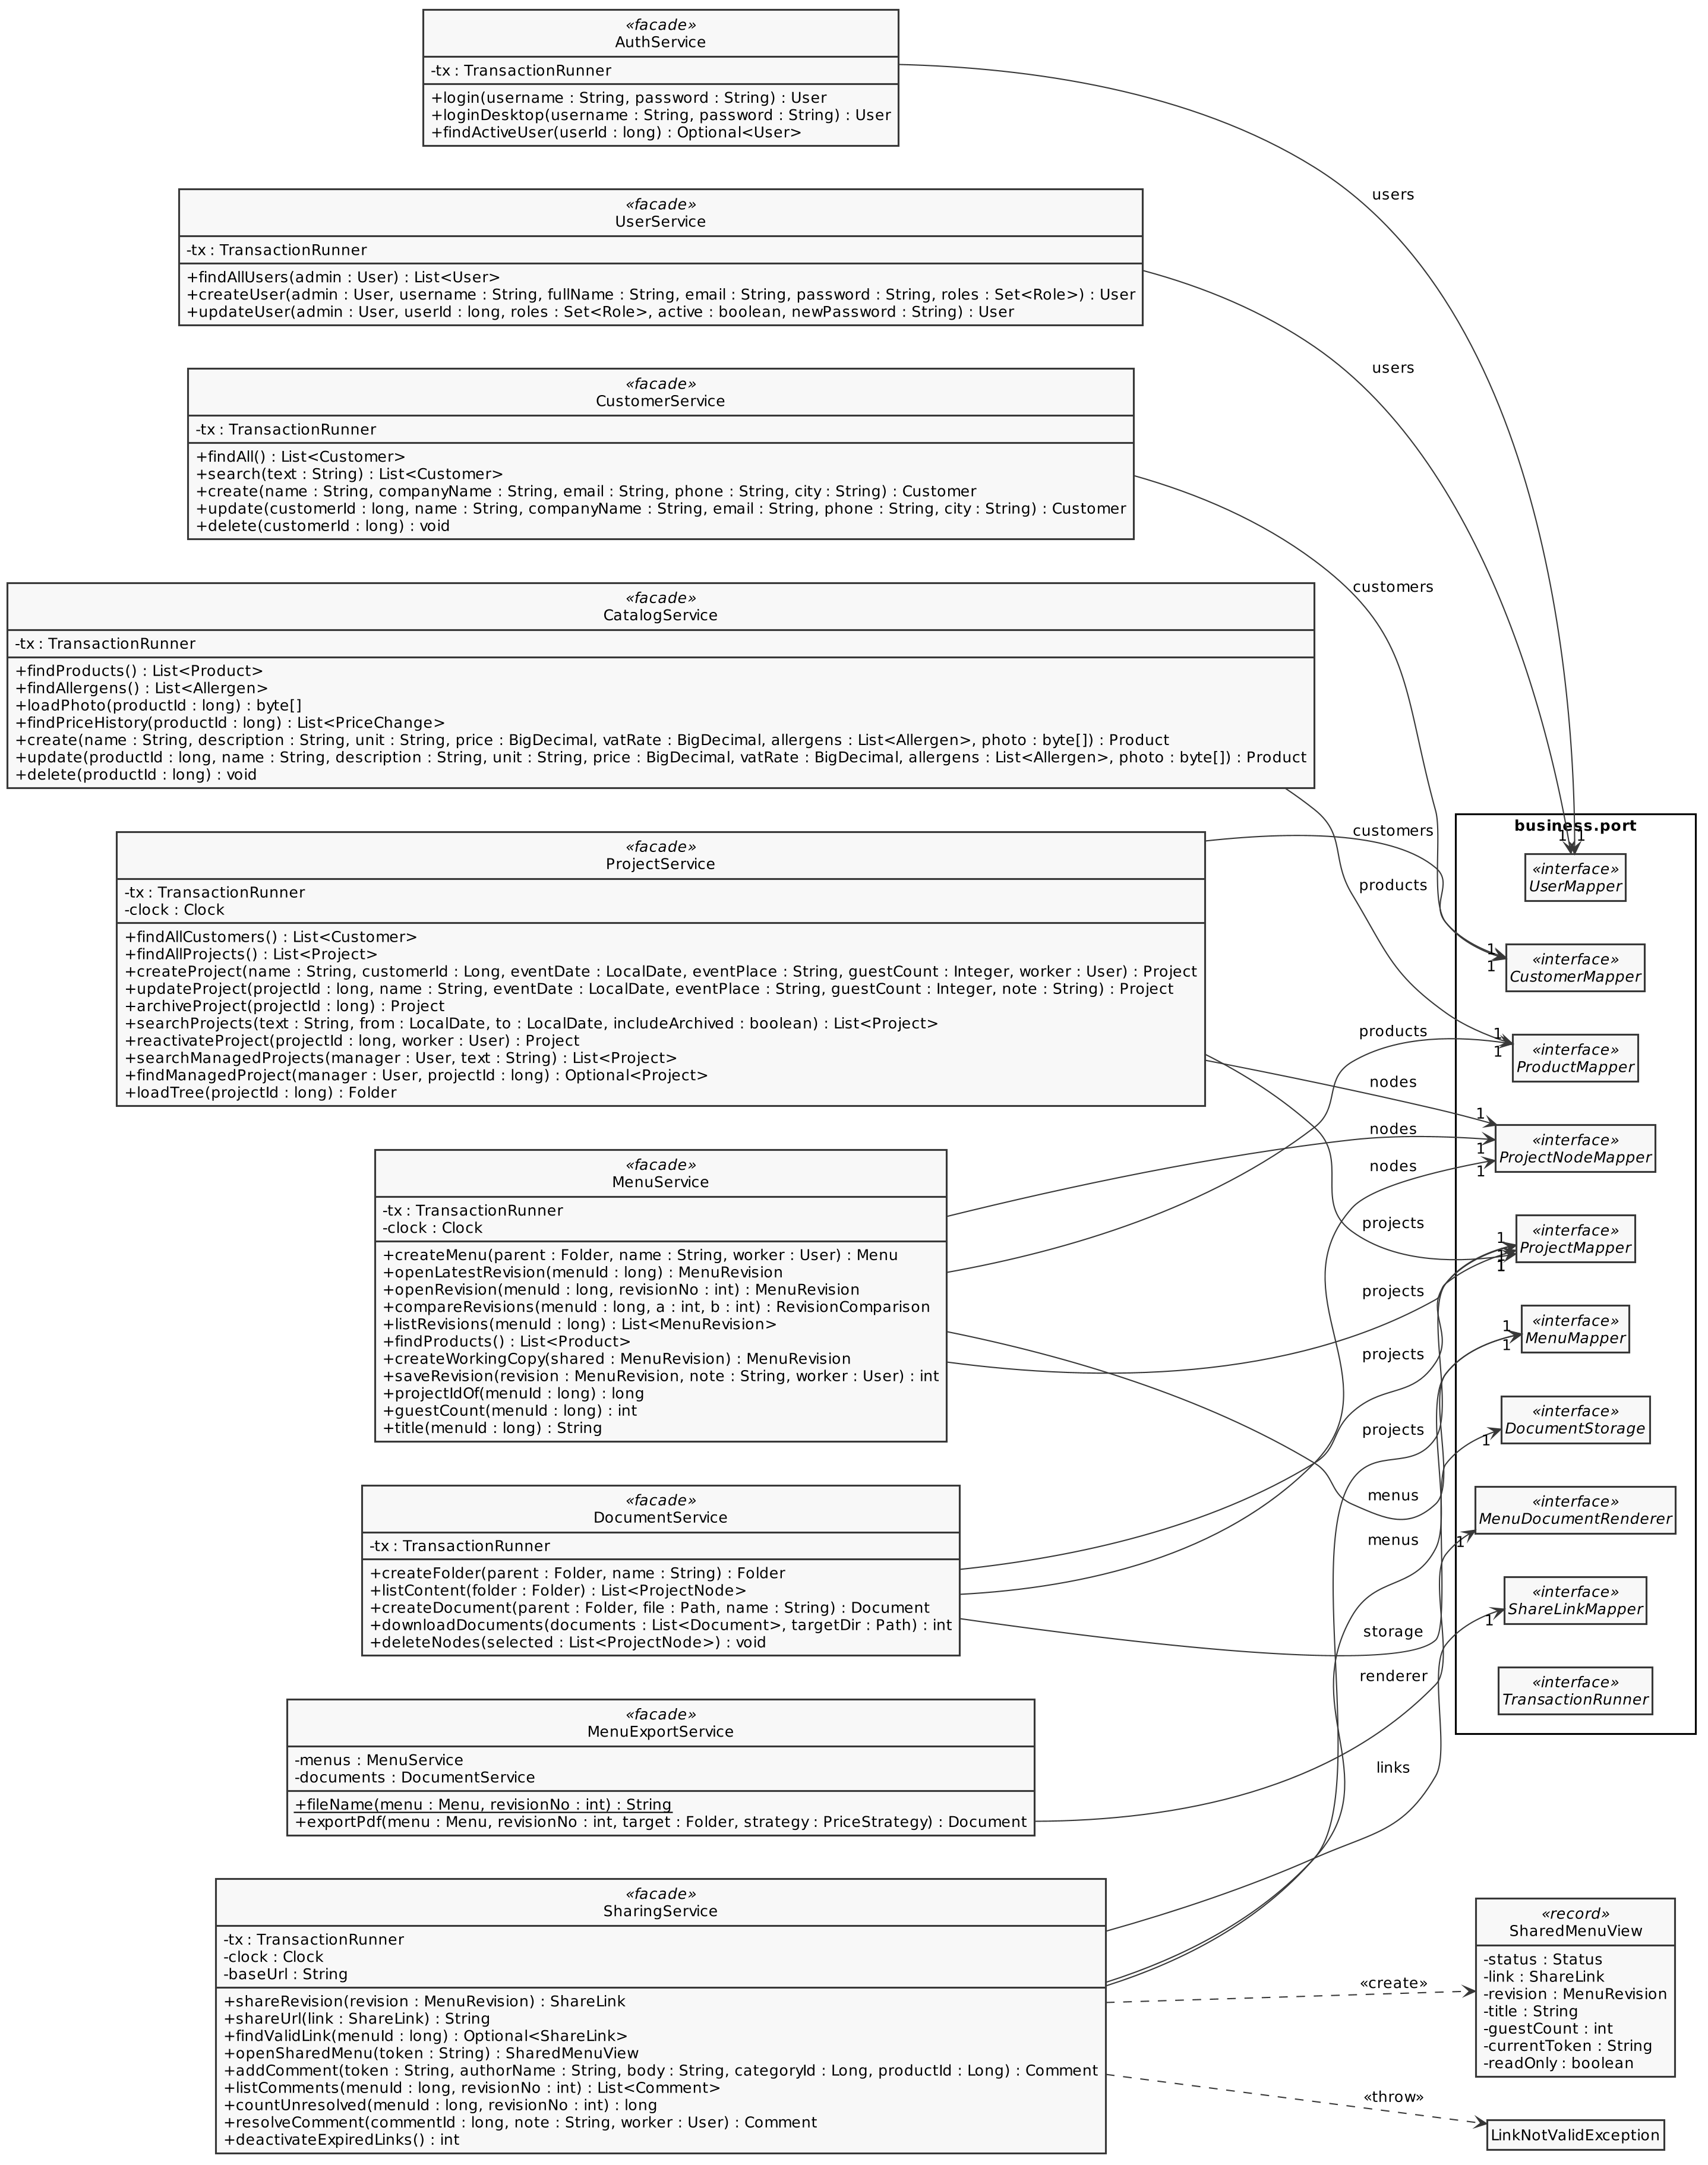
\includegraphics[width=\textwidth,height=0.85\textheight,keepaspectratio]{class-services.png}
  \caption{Diagram tříd -- aplikační služby (fasády) a rozhraní datové vrstvy}
  \label{fig:a5:services}
\end{figure}
\clearpage

\subsubsection*{Aplikační služby (\texttt{business.service})}

Služby na \odkaz{fig:a5:services}{obrázku služeb} tvoří rozhraní aplikační vrstvy pro desktopovou i webovou aplikaci. Každá metoda služby odpovídá jednomu kroku případu užití a běží v jedné transakci přes \texttt{TransactionRunner}. Pravidla domény služba nechává na doménových objektech. Sama jen načte data přes mapper, zavolá doménovou metodu a výsledek uloží. Metody, které zakládají nebo mění data (\texttt{createProject}, \texttt{reactivateProject}, \texttt{createMenu}, \texttt{saveRevision}, \texttt{resolveComment}), dostávají uživatele a ověřují ho přes \texttt{AccessPolicy.requireWorker}. Ostatní metody bez parametru uživatele jsou chráněné přihlášením a nabídkou v uživatelském rozhraní.

\begin{description}[itemsep=2pt,style=unboxed]
  \item[\texttt{ProjectService}] Zakládání, úprava, archivace a obnovení (\texttt{reactivateProject}) projektů, vyhledávání a načtení stromu projektu (\ucref{02}, \ucref{03}, \ucref{04}). Metody \texttt{searchManagedProjects} a \texttt{findManagedProject} vracejí manažerovi jen projekty pracovníků, kteří mu podléhají (\ucref{15}).
  \item[\texttt{DocumentService}] Práce se stromem projektu. Vytváří složky, nahrává a stahuje dokumenty a maže vybrané uzly (\ucref{02}). Obsah souborů ukládá přes \texttt{DocumentStorage}.
  \item[\texttt{MenuService}] Založení menu, otevření a porovnání revizí, vytvoření pracovní kopie a uložení revize s kontrolou souběžné změny (\ucref{08}). Pracovní kopii odmítne, dokud je nejnovější revize pracovní. Metoda \texttt{projectIdOf} zjistí projekt menu, aby webová stránka manažera ověřila oprávnění.
  \item[\texttt{MenuExportService}] Vytvoří PDF z revize menu a uloží ho jako dokument do vybrané složky projektu.
  \item[\texttt{SharingService}] Sdílení revize odkazem, otevření sdíleného menu zákazníkem, přidání a vyřízení komentářů a zneplatnění prošlých odkazů (\ucref{11}, \ucref{13}).
  \item[\texttt{SharedMenuView}] Výsledek otevření sdíleného odkazu pro webovou stránku. Obsahuje stav odkazu, revizi, název a počet hostů.
  \item[\texttt{LinkNotValidException}] Výjimka pro komentář přes odkaz, který už neplatí.
  \item[\texttt{CatalogService}] Správa katalogu produktů, alergenů, fotografií a historie cen.
  \item[\texttt{CustomerService}] Správa zákazníků. Zákazníka s projekty nelze smazat.
  \item[\texttt{AuthService}] Přihlášení uživatele jménem a heslem (\texttt{login}). Metoda \texttt{loginDesktop} navíc pustí do desktopové aplikace jen pracovníka nebo administrátora. Metoda \texttt{findActiveUser} znovu načte aktivního uživatele podle identifikátoru a používá ji webová relace manažera při každém požadavku.
  \item[\texttt{UserService}] Správa uživatelů a jejich rolí administrátorem (\ucref{16}). Hlídá, aby zůstal aspoň jeden aktivní administrátor. Oprávnění volajícího ověřuje čerstvým načtením z databáze, ne podle objektu z přihlášení.
\end{description}

\clearpage
\begin{figure}[H]
  \centering
  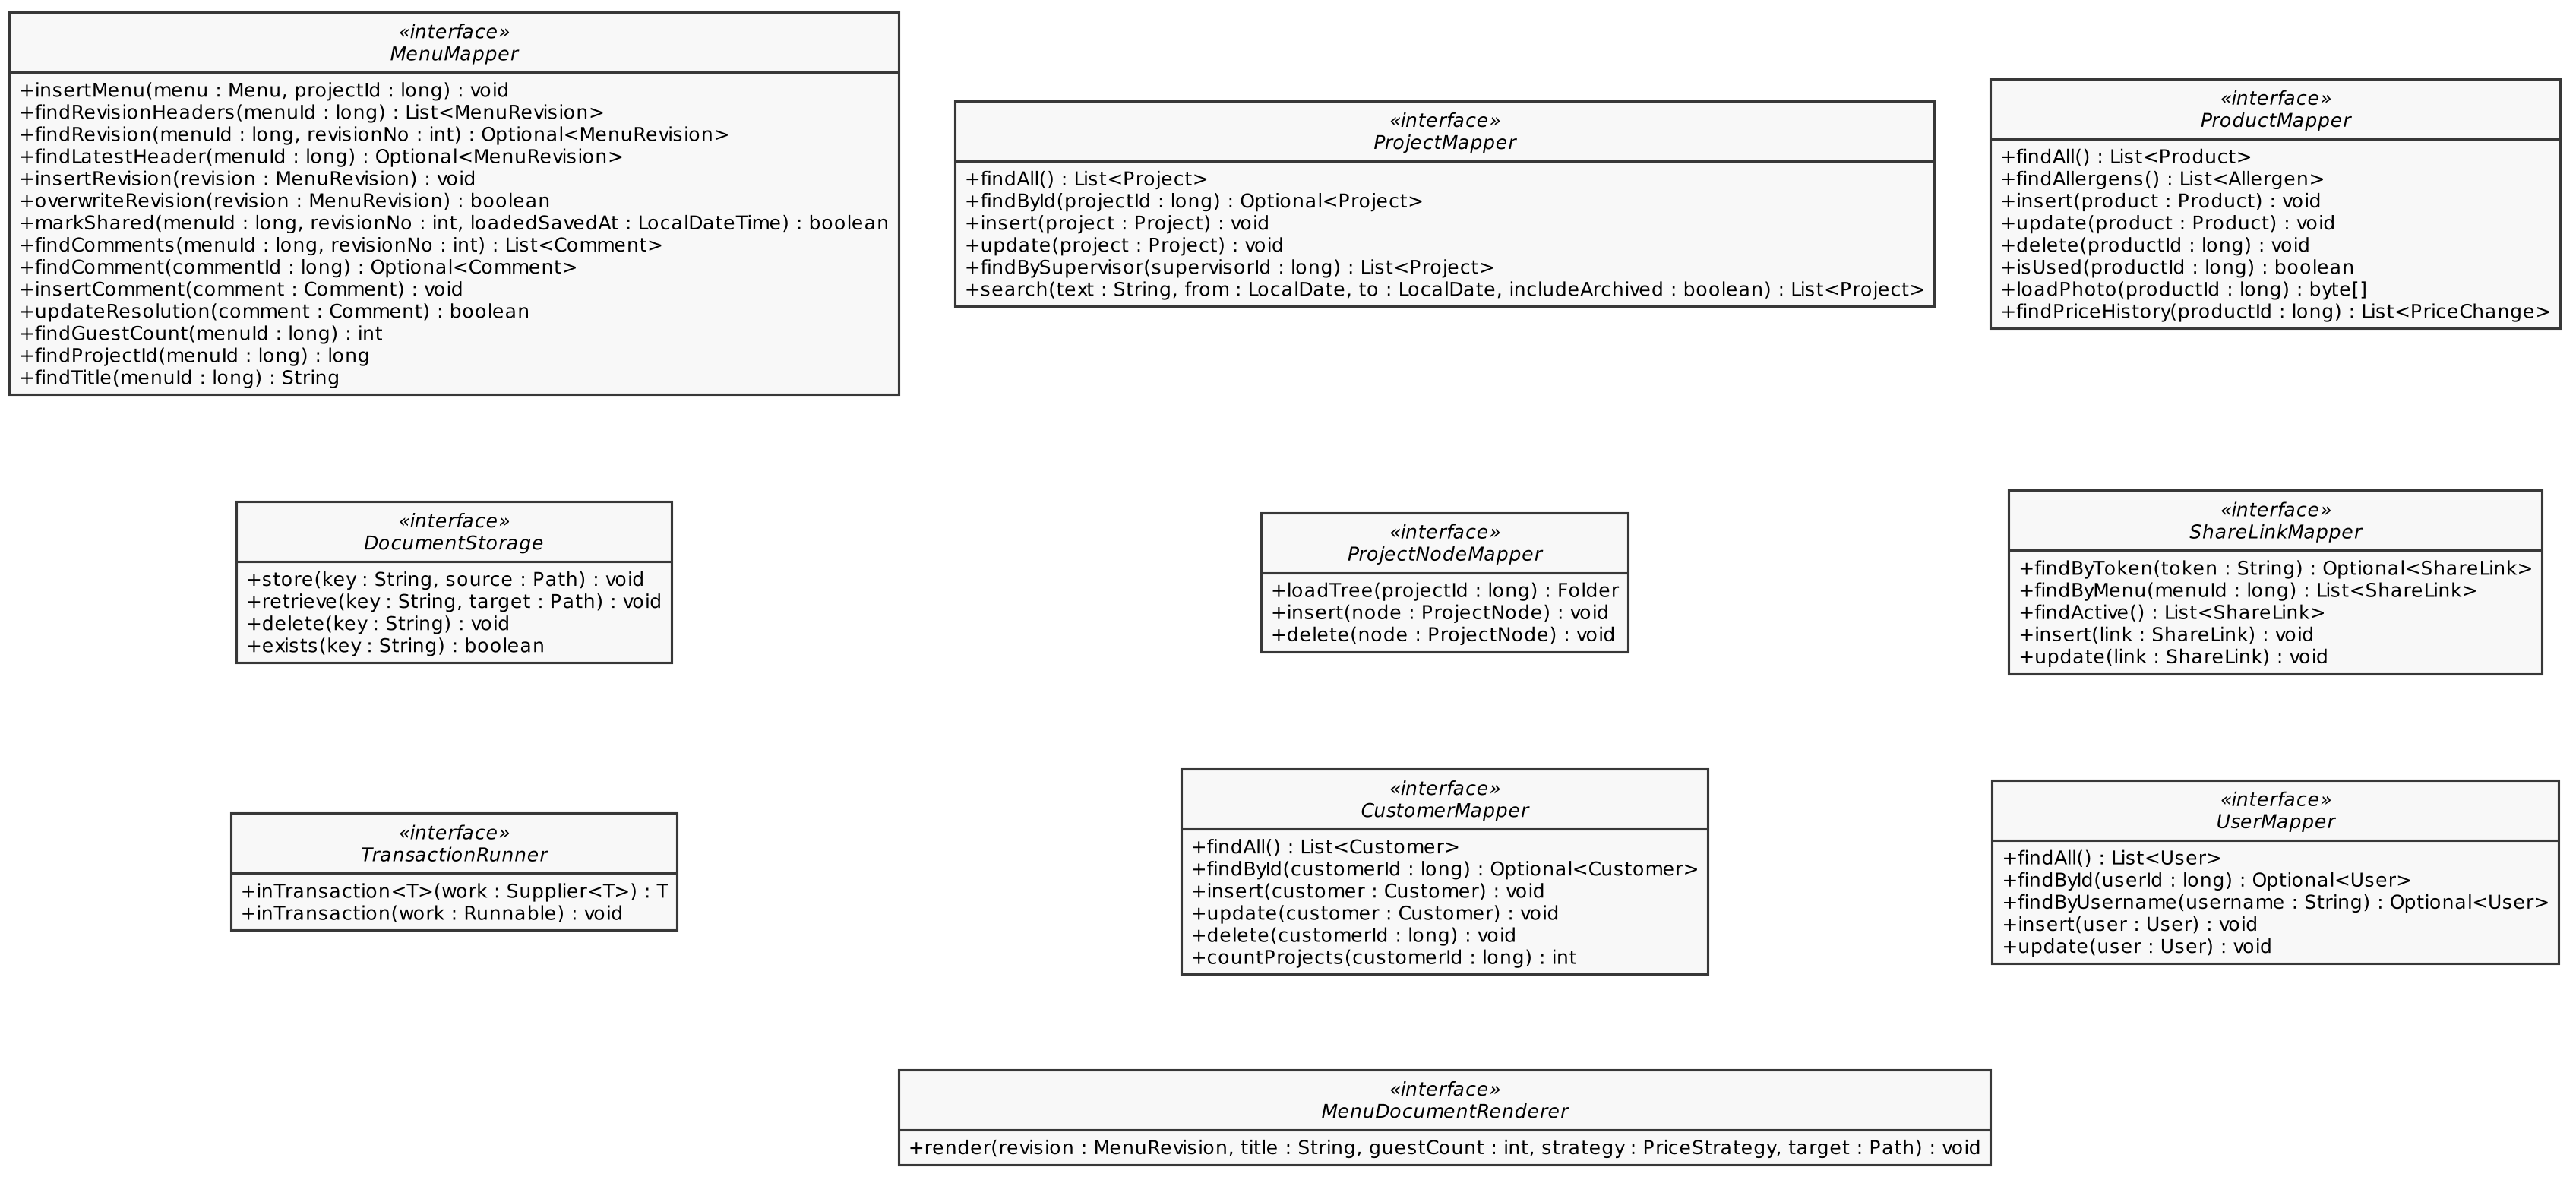
\includegraphics[width=0.85\textheight,height=\textwidth,keepaspectratio,angle=90]{class-ports.png}
  \caption{Diagram tříd -- rozhraní pro přístup k datům (\texttt{business.port})}
  \label{fig:a5:ports}
\end{figure}
\clearpage

\subsubsection*{Rozhraní pro přístup k datům (\texttt{business.port})}

Rozhraní na \odkaz{fig:a5:ports}{obrázku rozhraní} definuje aplikační vrstva a implementuje je datová vrstva (Dependency Inversion). Aplikační vrstva proto nezávisí na JDBC, SQL ani na souborech. Metody pracují s doménovými objekty.

\begin{description}[itemsep=2pt,style=unboxed]
  \item[\texttt{ProjectMapper}] Načtení, uložení a vyhledávání projektů včetně jejich zákazníka. Metoda \texttt{findBySupervisor} vrací projekty, jejichž odpovědný pracovník podléhá danému manažerovi.
  \item[\texttt{ProjectNodeMapper}] Načtení celého stromu projektu, vložení a smazání uzlu.
  \item[\texttt{MenuMapper}] Menu, revize s kategoriemi a položkami a komentáře. Metoda \texttt{overwriteRevision} přepíše jen pracovní revizi a vrací \texttt{false}, když ji mezitím uložil nebo sdílel někdo jiný. Metoda \texttt{markShared} změní pracovní revizi na sdílenou za stejné podmínky a také vrací \texttt{false} při souběžné změně.
  \item[\texttt{ProductMapper}] Katalog produktů, alergeny, fotografie a historie cen.
  \item[\texttt{CustomerMapper}] Zákazníci a počet jejich projektů.
  \item[\texttt{ShareLinkMapper}] Sdílené odkazy podle tokenu nebo menu a seznam aktivních odkazů.
  \item[\texttt{UserMapper}] Uživatelé včetně rolí.
  \item[\texttt{DocumentStorage}] Druhé úložiště pro obsah dokumentů. Ukládá, čte a maže soubor podle klíče.
  \item[\texttt{MenuDocumentRenderer}] Vykreslí revizi menu do tisknutelného dokumentu.
  \item[\texttt{TransactionRunner}] Spustí práci v jedné databázové transakci. Při výjimce provede rollback.
\end{description}

\clearpage
\begin{figure}[H]
  \centering
  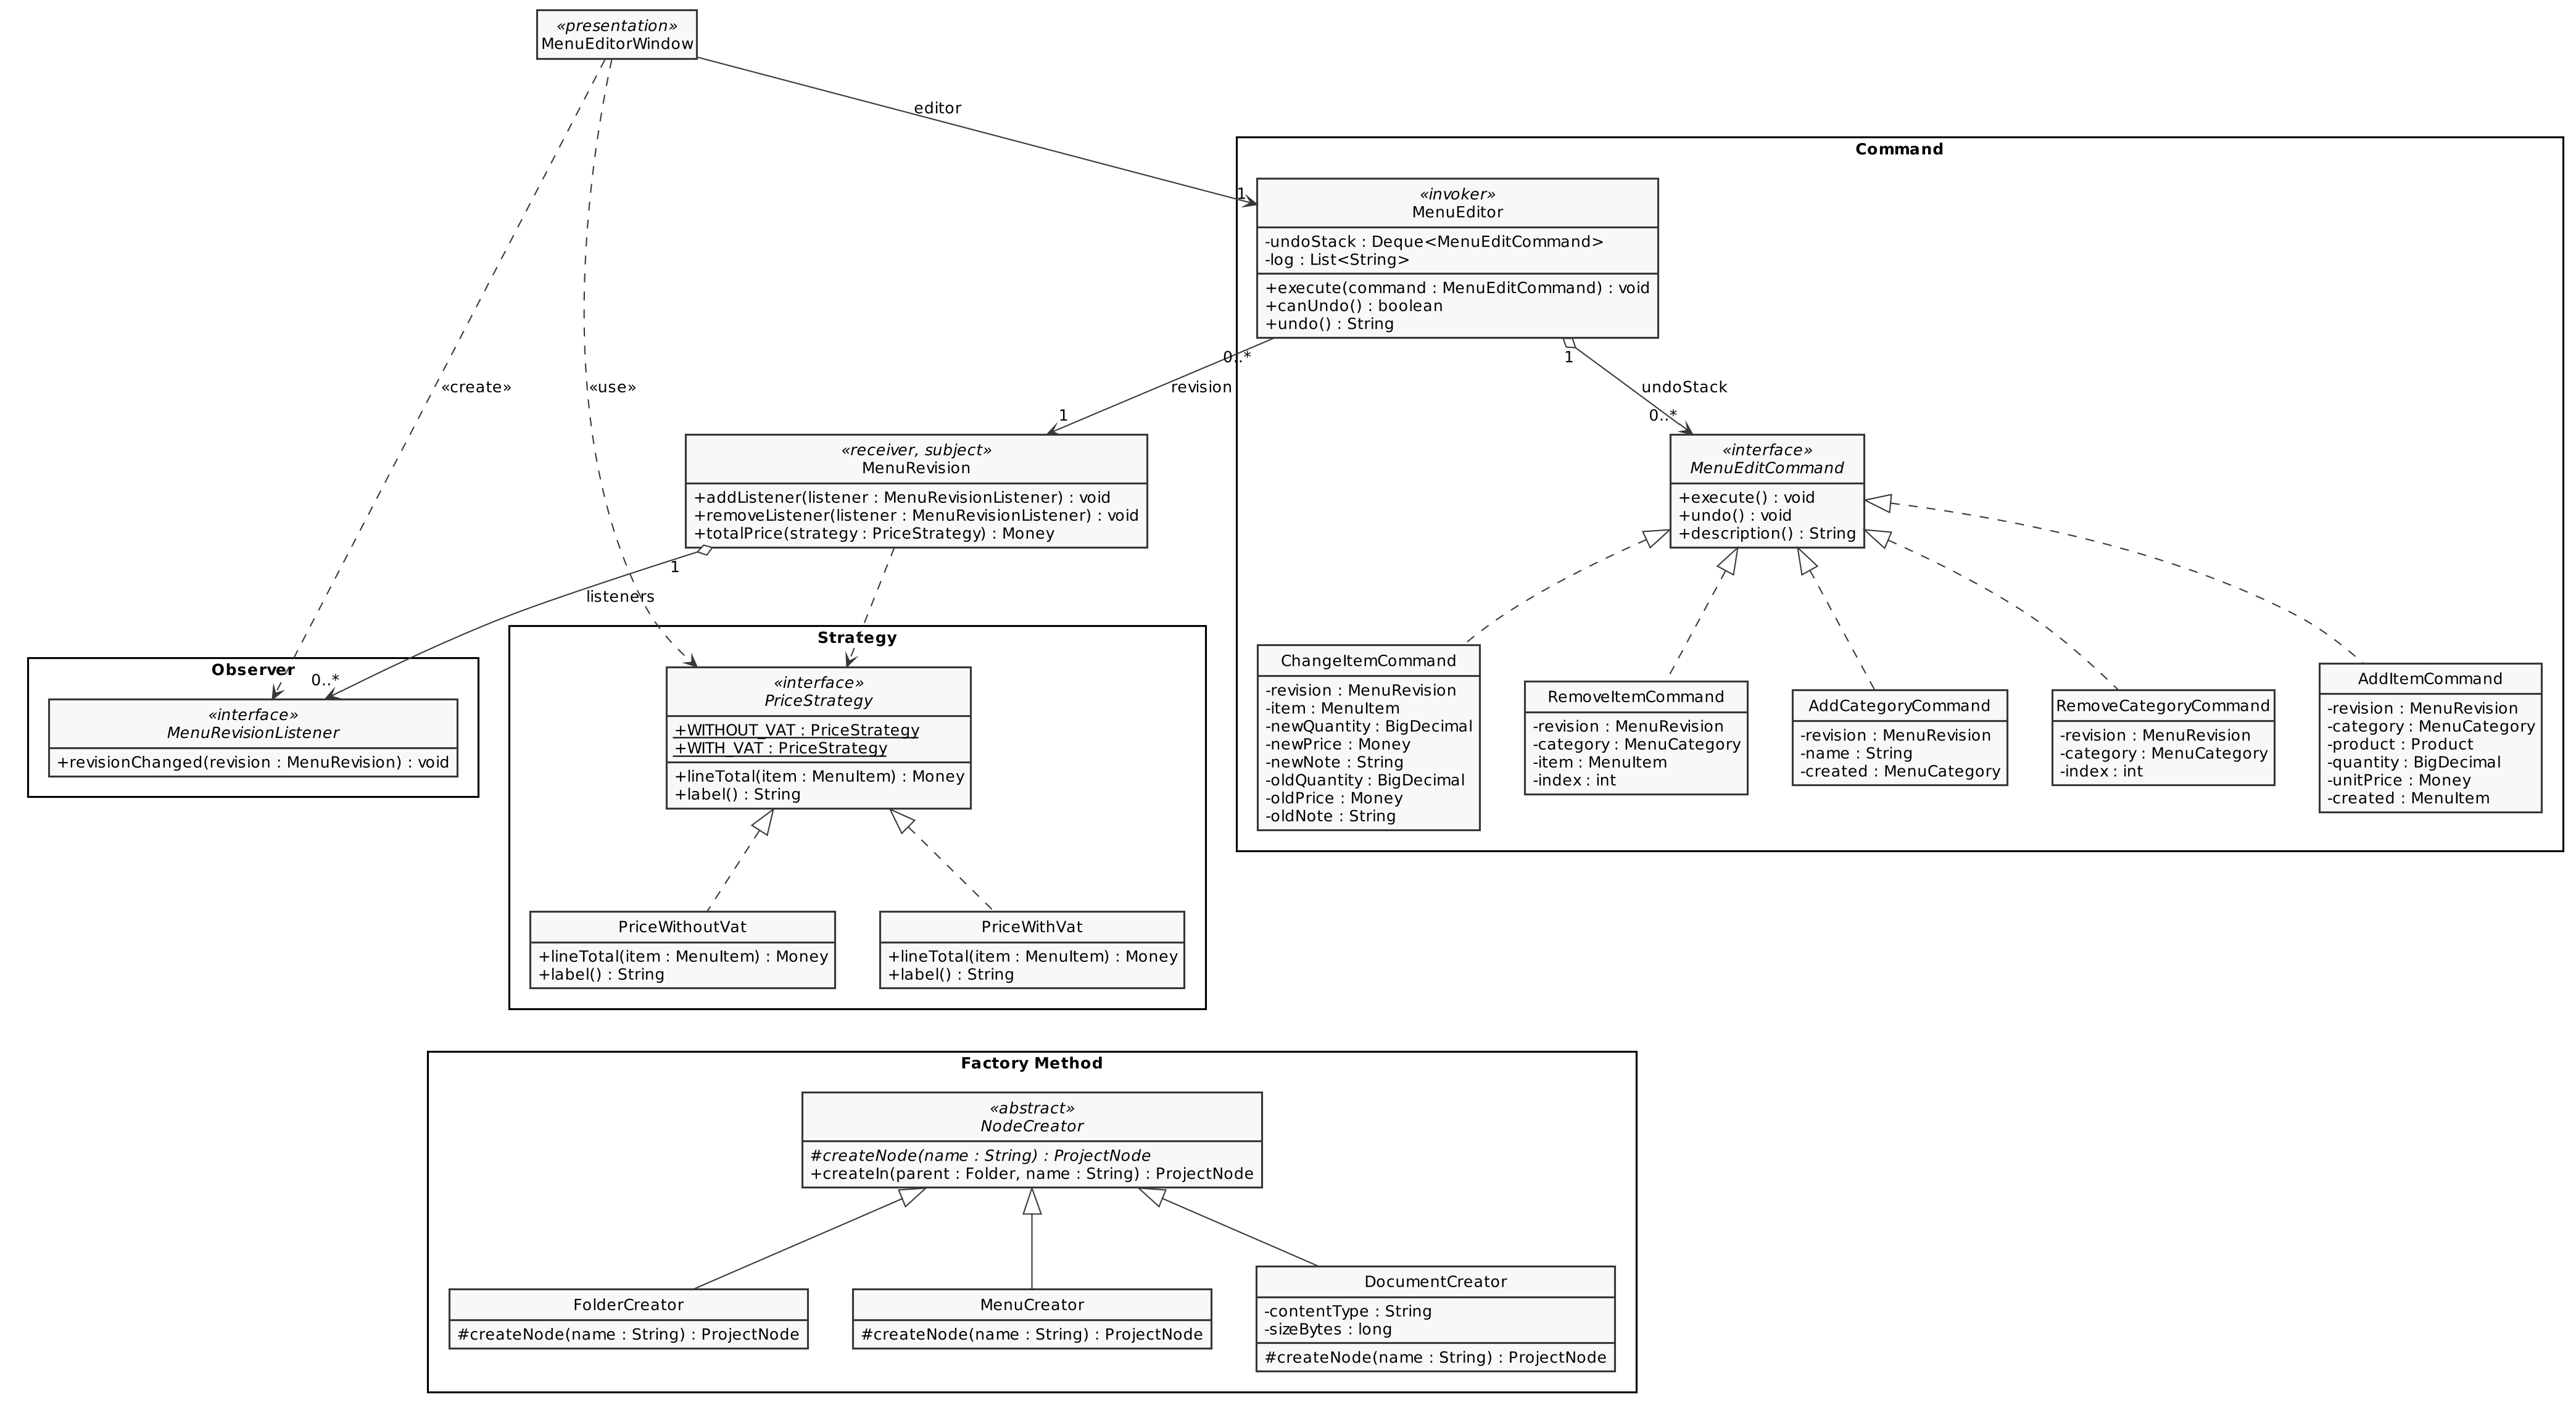
\includegraphics[width=0.85\textheight,height=\textwidth,keepaspectratio,angle=90]{class-gof.png}
  \caption{Diagram tříd -- vzory Command, Observer, Strategy a Factory Method}
  \label{fig:a5:gof}
\end{figure}
\clearpage

\subsubsection*{Vzory chování a vytváření (\texttt{business.command}, \texttt{business.pricing}, \texttt{business.domain})}

Obrázek \odkaz{fig:a5:gof}{diagram vzorů GoF} ukazuje třídy, které realizují úpravy menu s funkcí Zpět, výpočet ceny a vytváření uzlů stromu. Třída \texttt{MenuEditorWindow} z prezentační vrstvy je v diagramu jen jako klient, který vzory používá.

\begin{description}[itemsep=2pt,style=unboxed]
  \item[\texttt{MenuEditCommand}] Rozhraní jedné úpravy menu. Úpravu umí provést, vrátit a popsat pro historii změn.
  \item[\texttt{MenuEditor}] Spouští úpravy jedné revize a ukládá je do zásobníku. Tlačítko Zpět vrací poslední úpravu. Vede také textový záznam provedených úprav.
  \item[\texttt{AddCategoryCommand}] Přidá kategorii do revize. Zpět ji odebere.
  \item[\texttt{RemoveCategoryCommand}] Odebere kategorii a zapamatuje si její pořadí. Zpět ji vrátí na stejné místo.
  \item[\texttt{AddItemCommand}] Přidá produkt do kategorie s množstvím a cenou. Zpět položku odebere.
  \item[\texttt{ChangeItemCommand}] Změní množství, cenu a poznámku položky. Zapamatuje si původní hodnoty pro vrácení.
  \item[\texttt{RemoveItemCommand}] Odebere položku z kategorie a zapamatuje si její pořadí pro vrácení.
  \item[\texttt{MenuRevisionListener}] Posluchač změn revize. Editor menu jím po každé změně obnoví tabulku, součty a tlačítka.
  \item[\texttt{PriceStrategy}] Rozhraní výpočtu ceny řádku menu. Konstanty \texttt{WITHOUT\_VAT} a \texttt{WITH\_VAT} nabízejí obě implementace.
  \item[\texttt{PriceWithoutVat}] Cena řádku bez DPH (jednotková cena krát množství).
  \item[\texttt{PriceWithVat}] Cena řádku s DPH podle sazby produktu.
  \item[\texttt{NodeCreator}] Abstraktní tvůrce uzlů stromu. Metoda \texttt{createIn} ověří název (odmítne lomítka, zpětná lomítka, řídicí znaky a názvy \texttt{.} a \texttt{..}) a vloží uzel do složky. Konkrétní uzel vytvoří tovární metoda \texttt{createNode} potomka.
  \item[\texttt{FolderCreator}, \texttt{MenuCreator}, \texttt{DocumentCreator}] Vnořené třídy \texttt{NodeCreator}, které vytvářejí složku, menu a dokument. \texttt{DocumentCreator} navíc kontroluje velikost souboru.
  \item[\texttt{MenuEditorWindow}] Okno editoru menu v prezentační vrstvě (\ucref{08}). Spouští příkazy přes \texttt{MenuEditor}, registruje posluchače a přepíná cenovou strategii.
\end{description}

\subsection{Diagram datové vrstvy}\label{sec:a5:dal}

Datová vrstva implementuje rozhraní z balíčku \texttt{business.port}. \odkaz{fig:a5:dal}{Diagram datové vrstvy} ukazuje jeden mapper do databáze, obě implementace druhého úložiště, vykreslení PDF a třídy pro připojení. Ostatní mappery (\texttt{OracleProjectMapper}, \texttt{OracleProjectNodeMapper}, \texttt{OracleProductMapper}, \texttt{OracleCustomerMapper}, \texttt{OracleShareLinkMapper} a \texttt{OracleUserMapper}) jsou postavené stejně jako \texttt{OracleMenuMapper}, a proto v diagramu nejsou. Aplikace nepoužívá DTO. Mappery vracejí přímo doménové objekty.

Datová vrstva neobsahuje logiku aplikace. Mappery jen převádějí objekty na řádky tabulek a zpět. Všechna rozhodnutí, například zda lze revizi upravit nebo zda je odkaz platný, dělají doménové třídy a služby.

\clearpage
\begin{figure}[H]
  \centering
  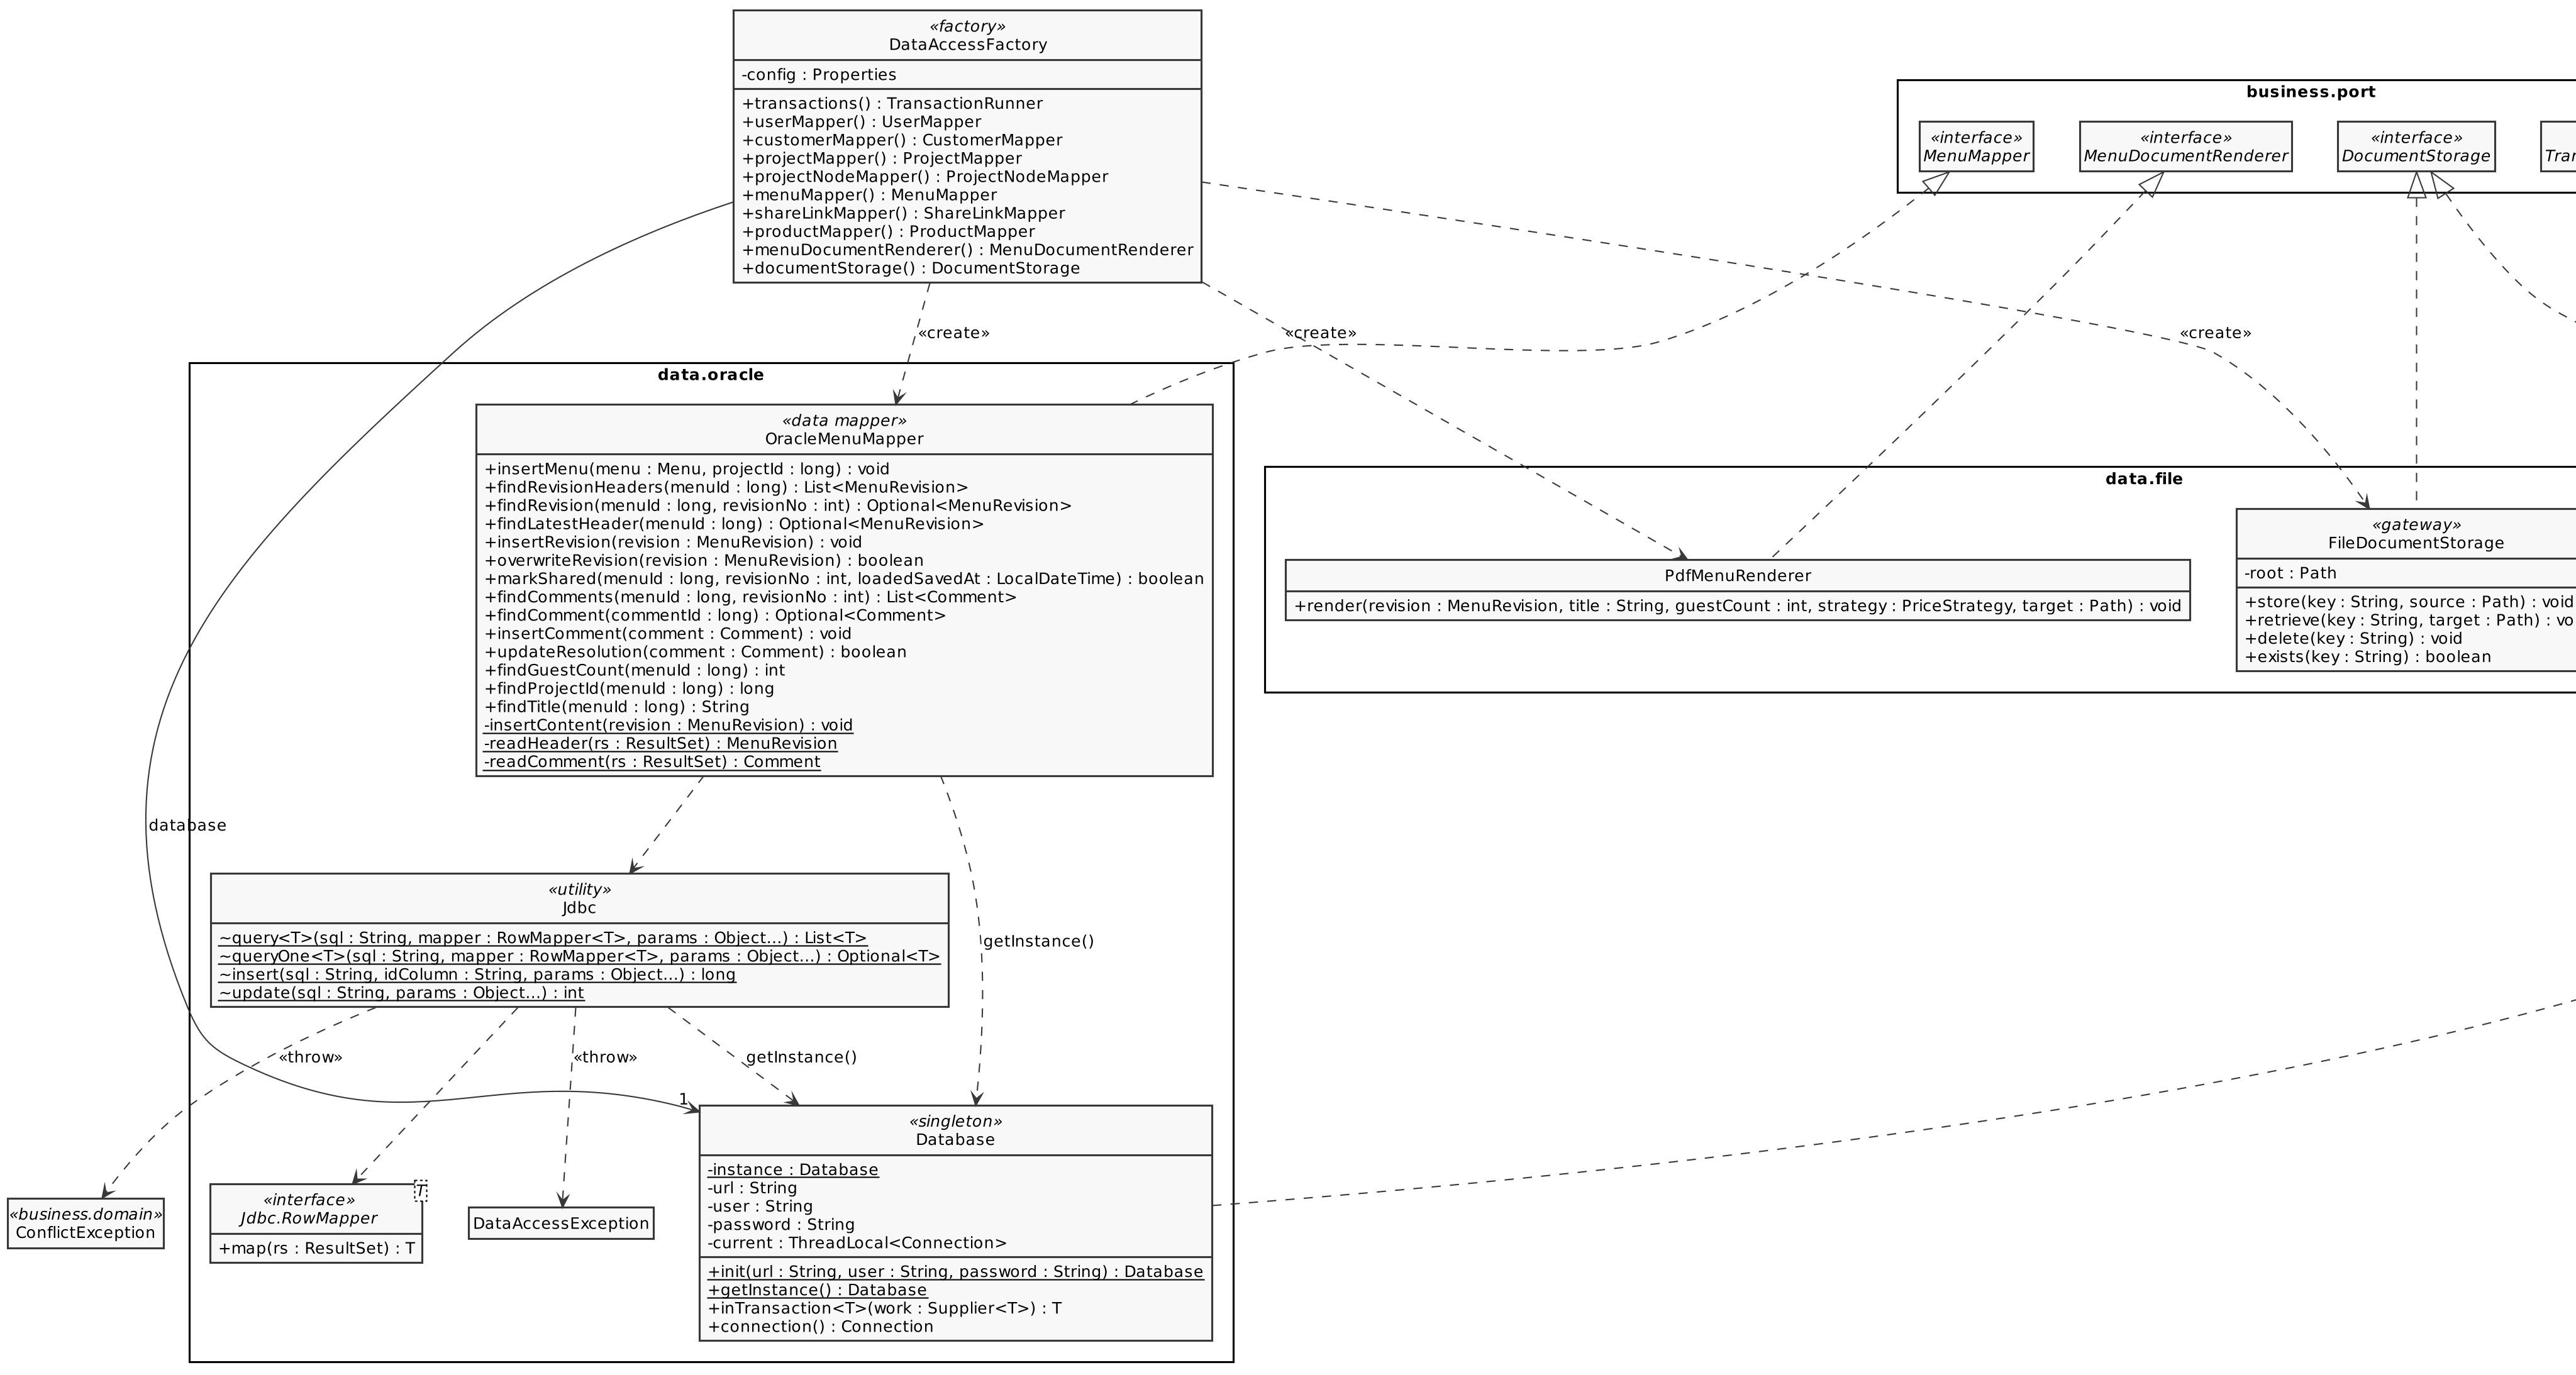
\includegraphics[width=0.85\textheight,height=\textwidth,keepaspectratio,angle=90]{class-dal.png}
  \caption{Diagram tříd datové vrstvy}
  \label{fig:a5:dal}
\end{figure}
\clearpage

\begin{description}[itemsep=2pt,style=unboxed]
  \item[\texttt{DataAccessFactory}] Podle konfiguračního souboru vytvoří připojení k databázi, všechny mappery, úložiště dokumentů a vykreslování PDF. Zbytek aplikace dostane jen rozhraní z \texttt{business.port}.
  \item[\texttt{Database}] Jediný poskytovatel připojení k databázi. Implementuje \texttt{TransactionRunner}. Pro každou transakci otevře spojení (s limitem 5 sekund na přihlášení), drží ho pro aktuální vlákno a na konci provede commit, při výjimce rollback. Selže-li i rollback, přidá se jeho chyba k původní výjimce.
  \item[\texttt{Jdbc}] Pomocná třída mapperů. Naváže parametry na dotaz, převede řádky výsledku na objekty přes \texttt{RowMapper} a vrátí vygenerovaný klíč nového řádku. Chybu SQL zabalí do \texttt{DataAccessException}, porušení jedinečnosti nebo primárního klíče převede na \texttt{ConflictException}, protože znamená, že byl rychlejší jiný pracovník.
  \item[\texttt{Jdbc.RowMapper}] Rozhraní pro převod jednoho řádku výsledku dotazu na objekt.
  \item[\texttt{OracleMenuMapper}] Mapper menu, revizí, kategorií, položek a komentářů. Kategorie a položky ukládá spolu s revizí. Komentáře revize načítá až na požádání.
  \item[\texttt{DataAccessException}] Nekontrolovaná výjimka, která nahrazuje \texttt{SQLException}, aby aplikační vrstva nezávisela na JDBC.
  \item[\texttt{FileDocumentStorage}] Ukládá obsah dokumentů jako soubory v adresáři z konfigurace. Klíč je relativní cesta a klíč mimo kořenový adresář odmítne. Soubor nejdřív zapíše do dočasného souboru a potom ho atomicky přesune, takže se nikdy neukáže rozepsaný.
  \item[\texttt{InMemoryDocumentStorage}] Náhrada úložiště, která drží soubory v paměti. Používají ji testy služeb, aby nepotřebovaly skutečný adresář.
  \item[\texttt{PdfMenuRenderer}] Vykreslí revizi menu do PDF knihovnou Apache PDFBox se zabudovaným písmem s českými znaky.
\end{description}

\subsection{Sekvenční diagramy}\label{sec:a5:seq}

Sekvenční diagramy zachycují interakci uživatele se systémem pro podrobně popsané případy užití. Mezi uživatelem a aplikačními službami je objekt uživatelského rozhraní, který představuje prezentační vrstvu. Delší případy užití jsou rozdělené do více diagramů podle kroků scénáře.

\clearpage
\begin{figure}[H]
  \centering
  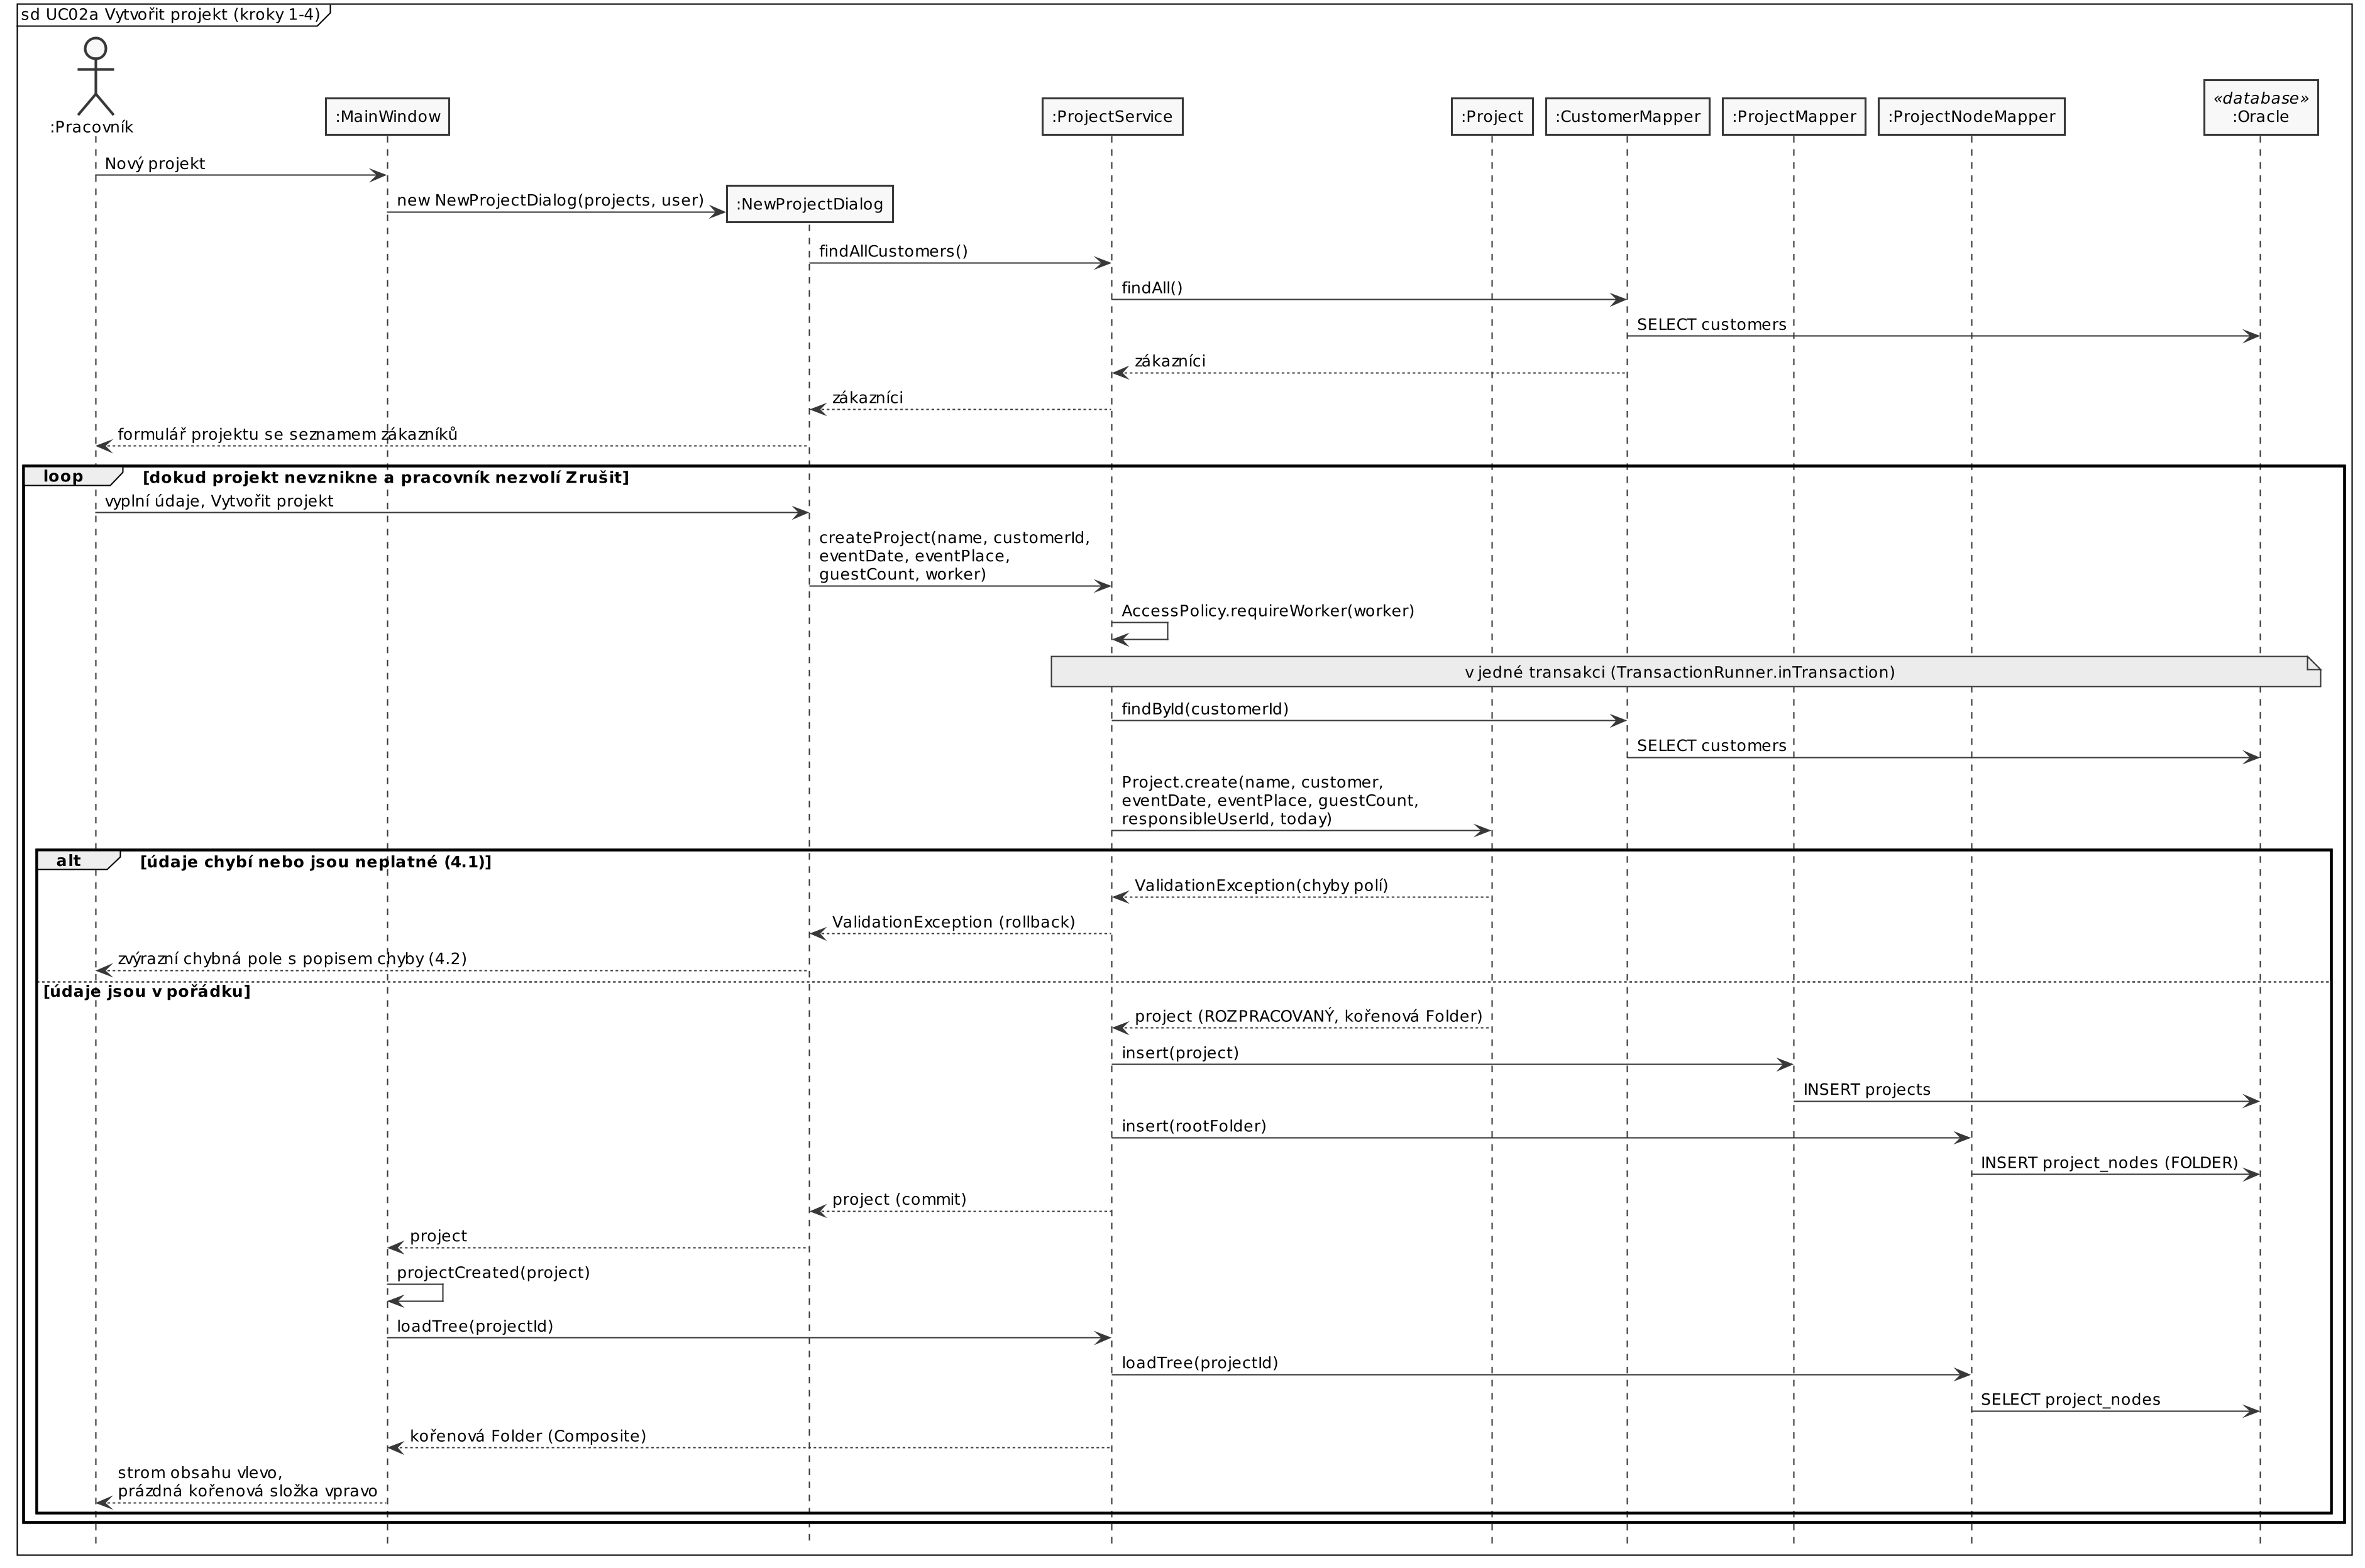
\includegraphics[width=\textwidth,height=0.85\textheight,keepaspectratio]{seq-uc02-a.png}
  \caption{Sekvenční diagram UC02 -- Vytvořit projekt (kroky 1--4, 4.1)}
\end{figure}
\clearpage

\begin{figure}[H]
  \centering
  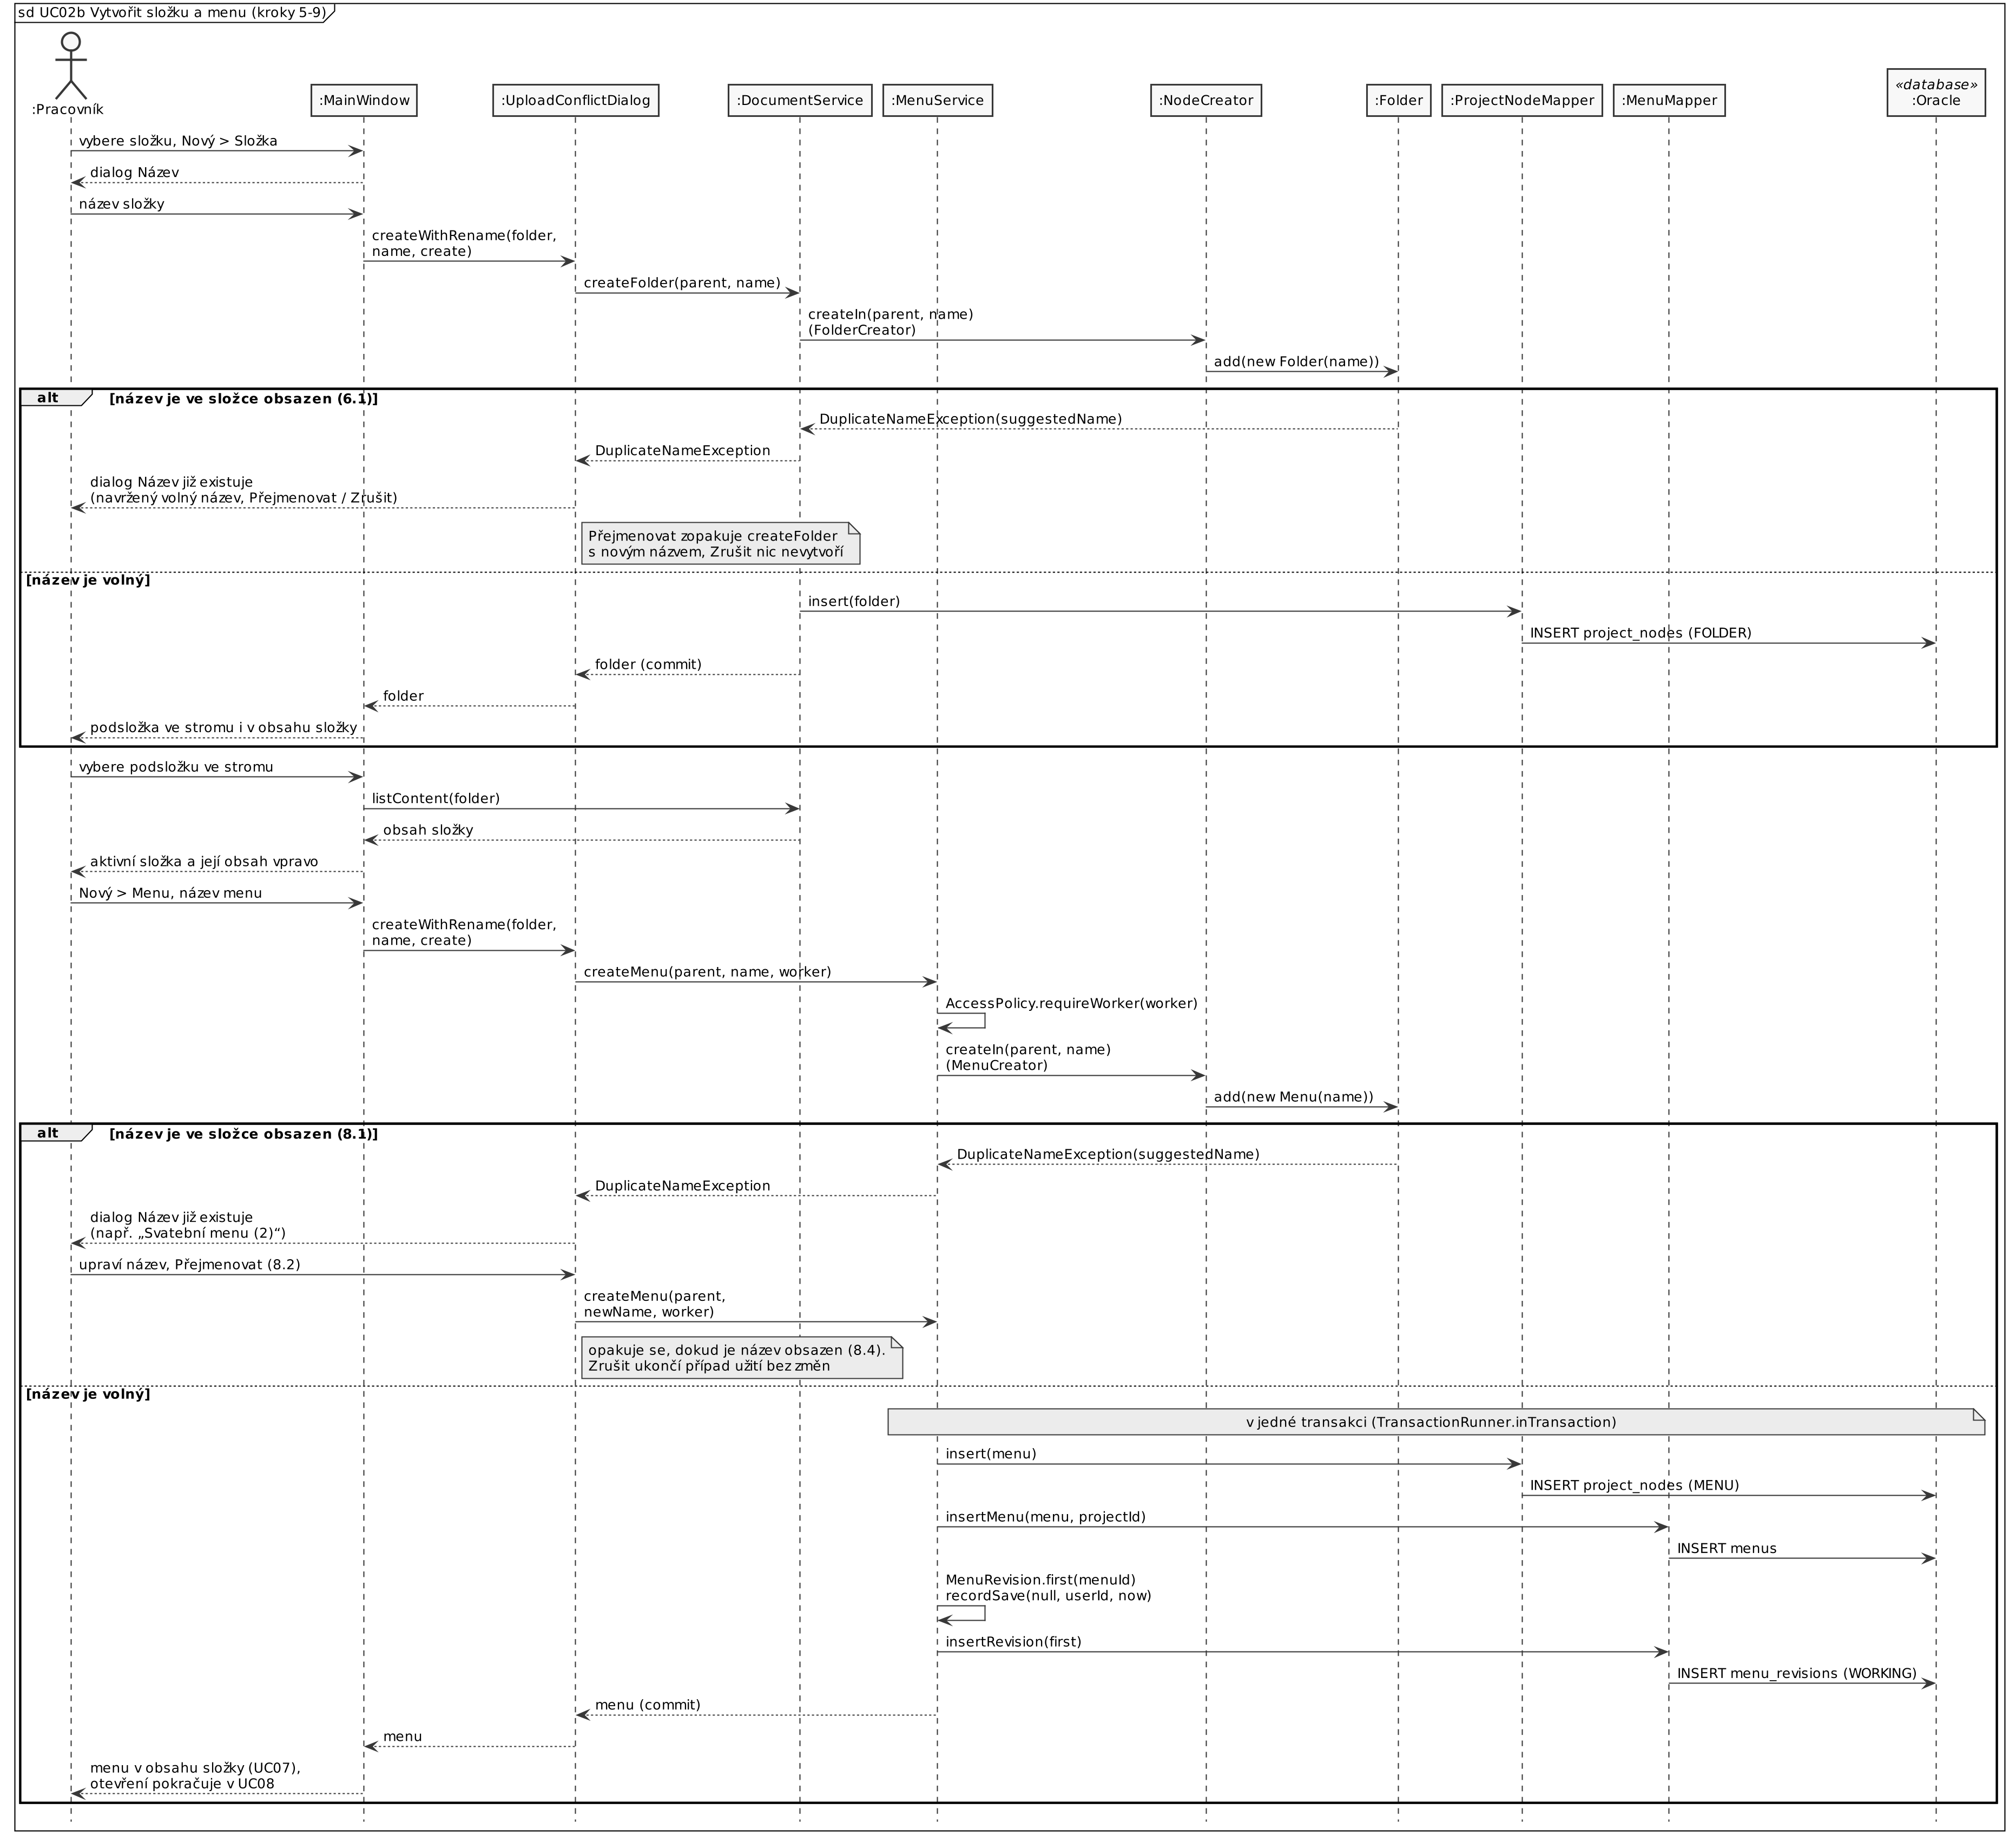
\includegraphics[width=\textwidth,height=0.85\textheight,keepaspectratio]{seq-uc02-b.png}
  \caption{Sekvenční diagram UC02 -- Spravovat strom projektu (kroky 5--9, 6.1, 8.1--8.5)}
\end{figure}
\clearpage

\begin{figure}[H]
  \centering
  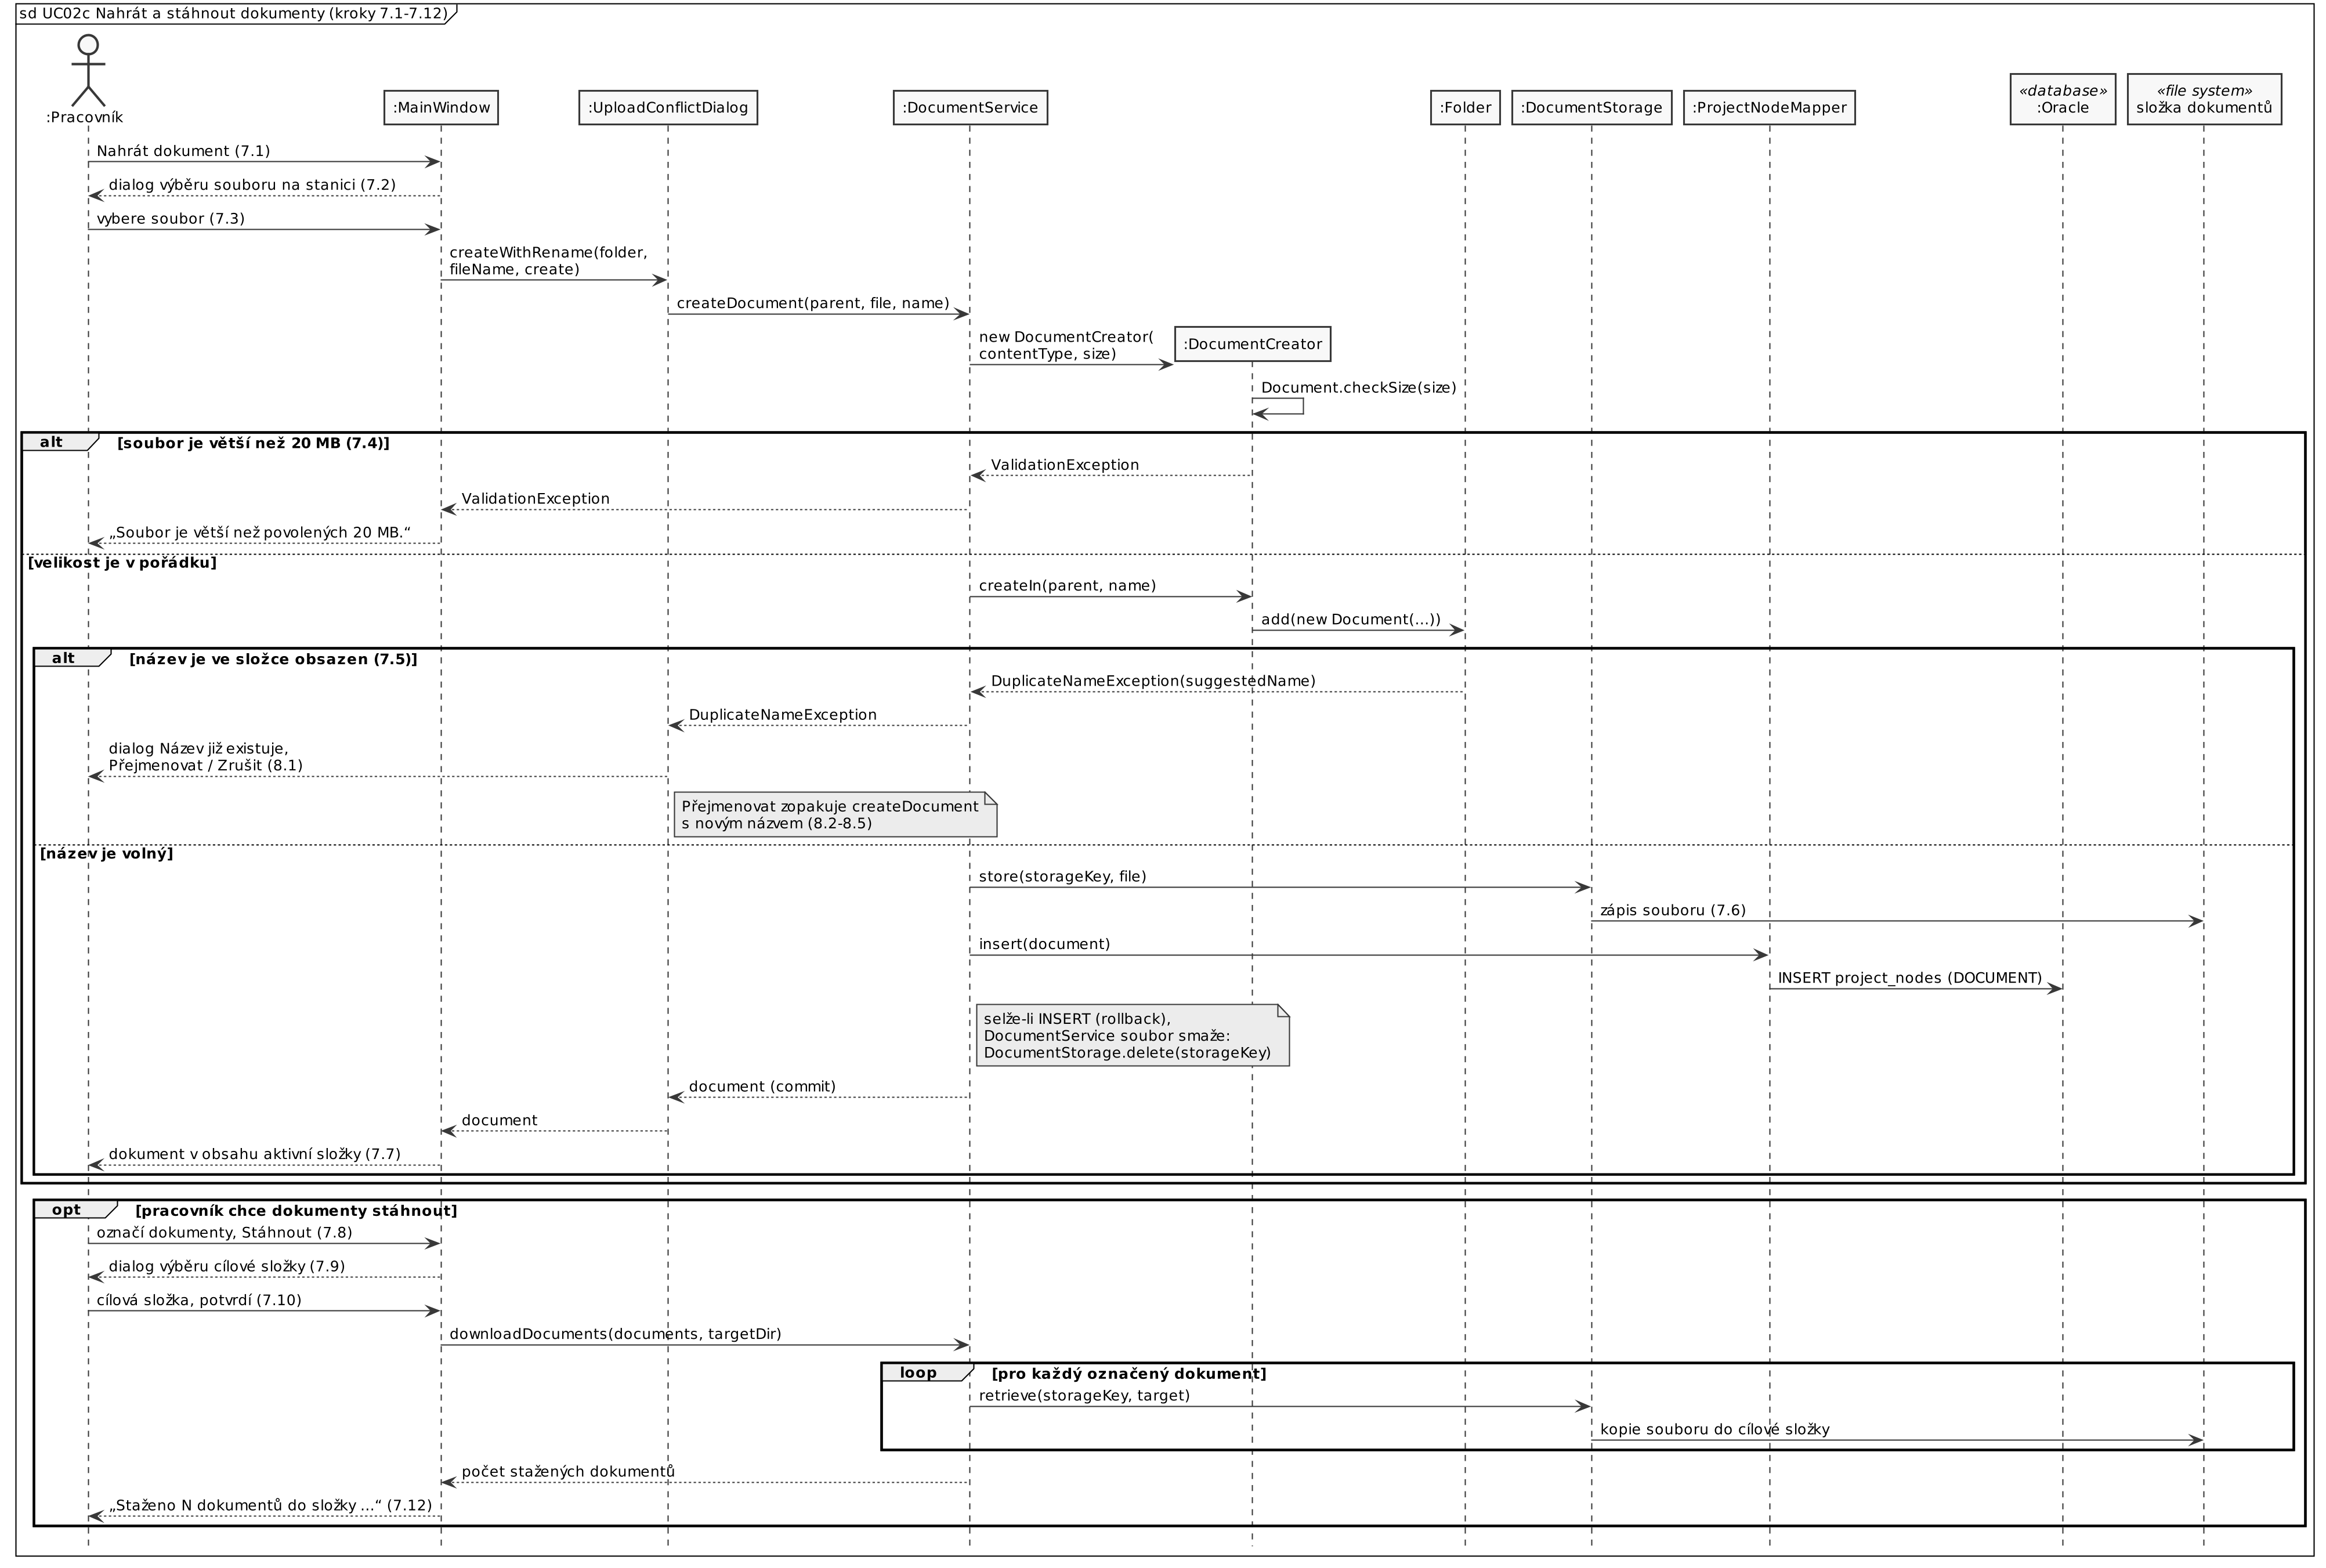
\includegraphics[width=\textwidth,height=0.85\textheight,keepaspectratio]{seq-uc02-c.png}
  \caption{Sekvenční diagram UC02 -- Nahrát a stáhnout dokument (kroky 7.1--7.12)}
\end{figure}
\clearpage

\begin{figure}[H]
  \centering
  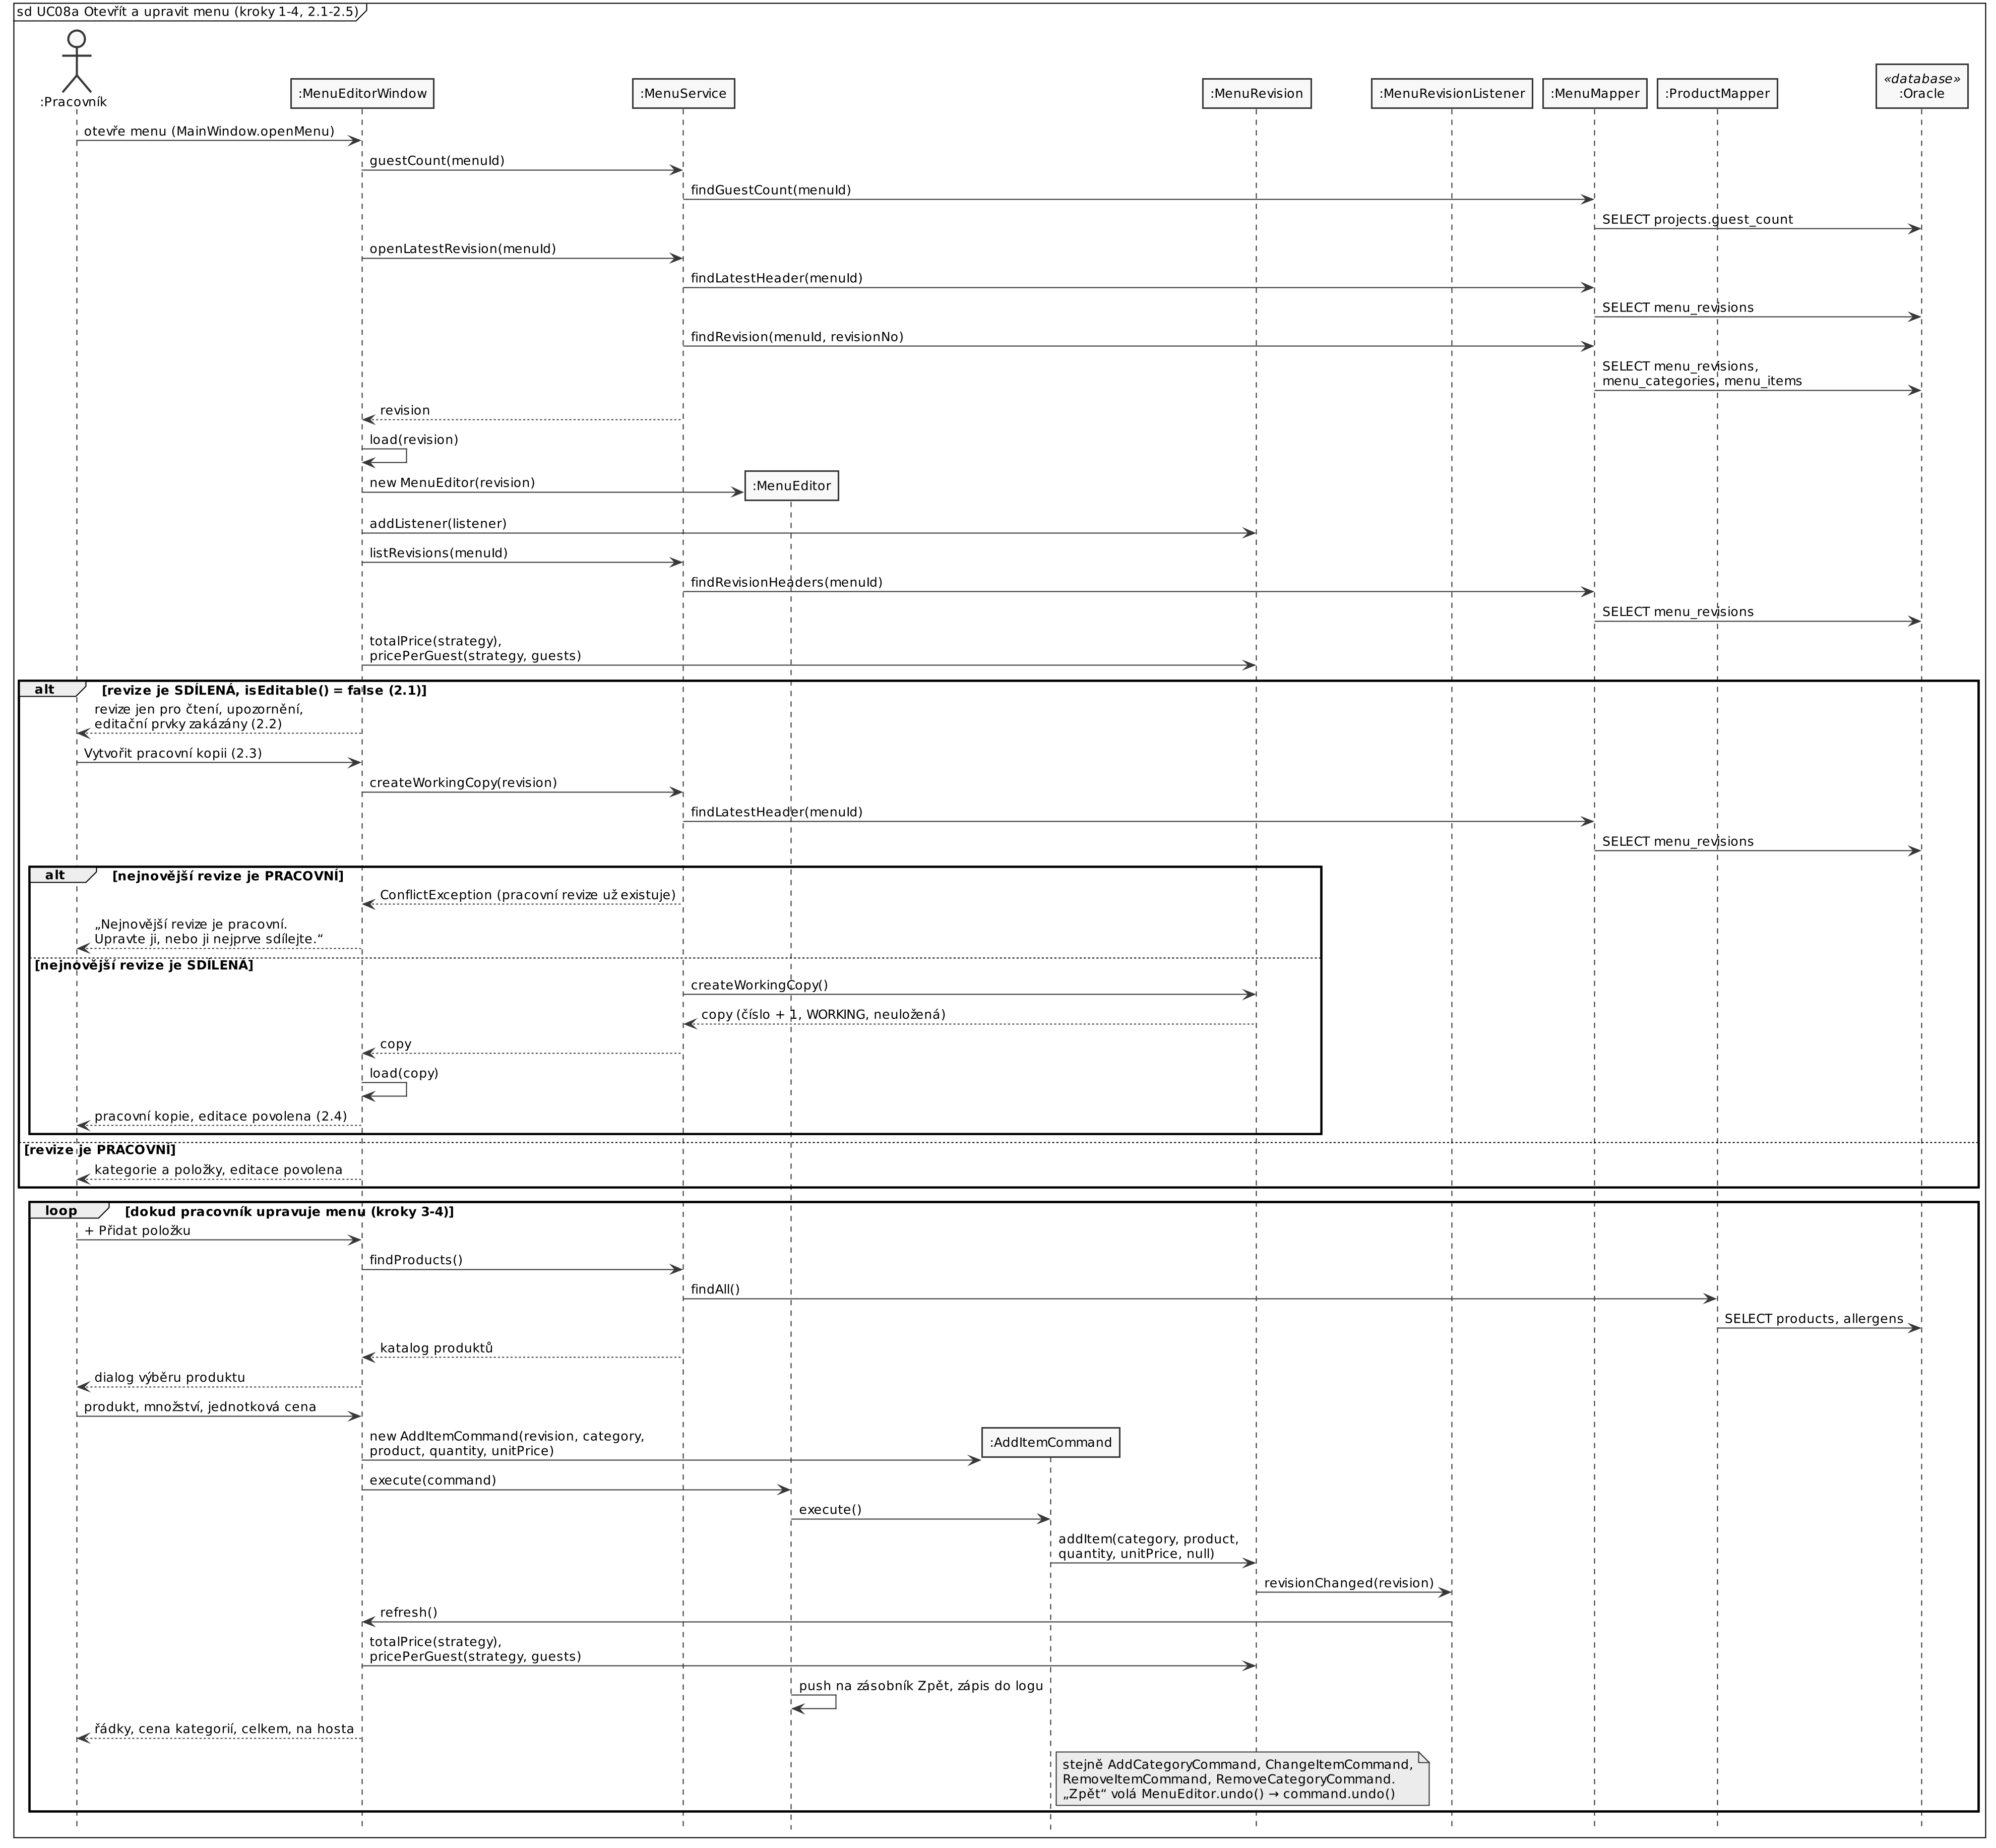
\includegraphics[width=\textwidth,height=0.85\textheight,keepaspectratio]{seq-uc08-a.png}
  \caption{Sekvenční diagram UC08 -- Otevřít a upravit menu (kroky 1--4, 2.1--2.5)}
\end{figure}
\clearpage

\begin{figure}[H]
  \centering
  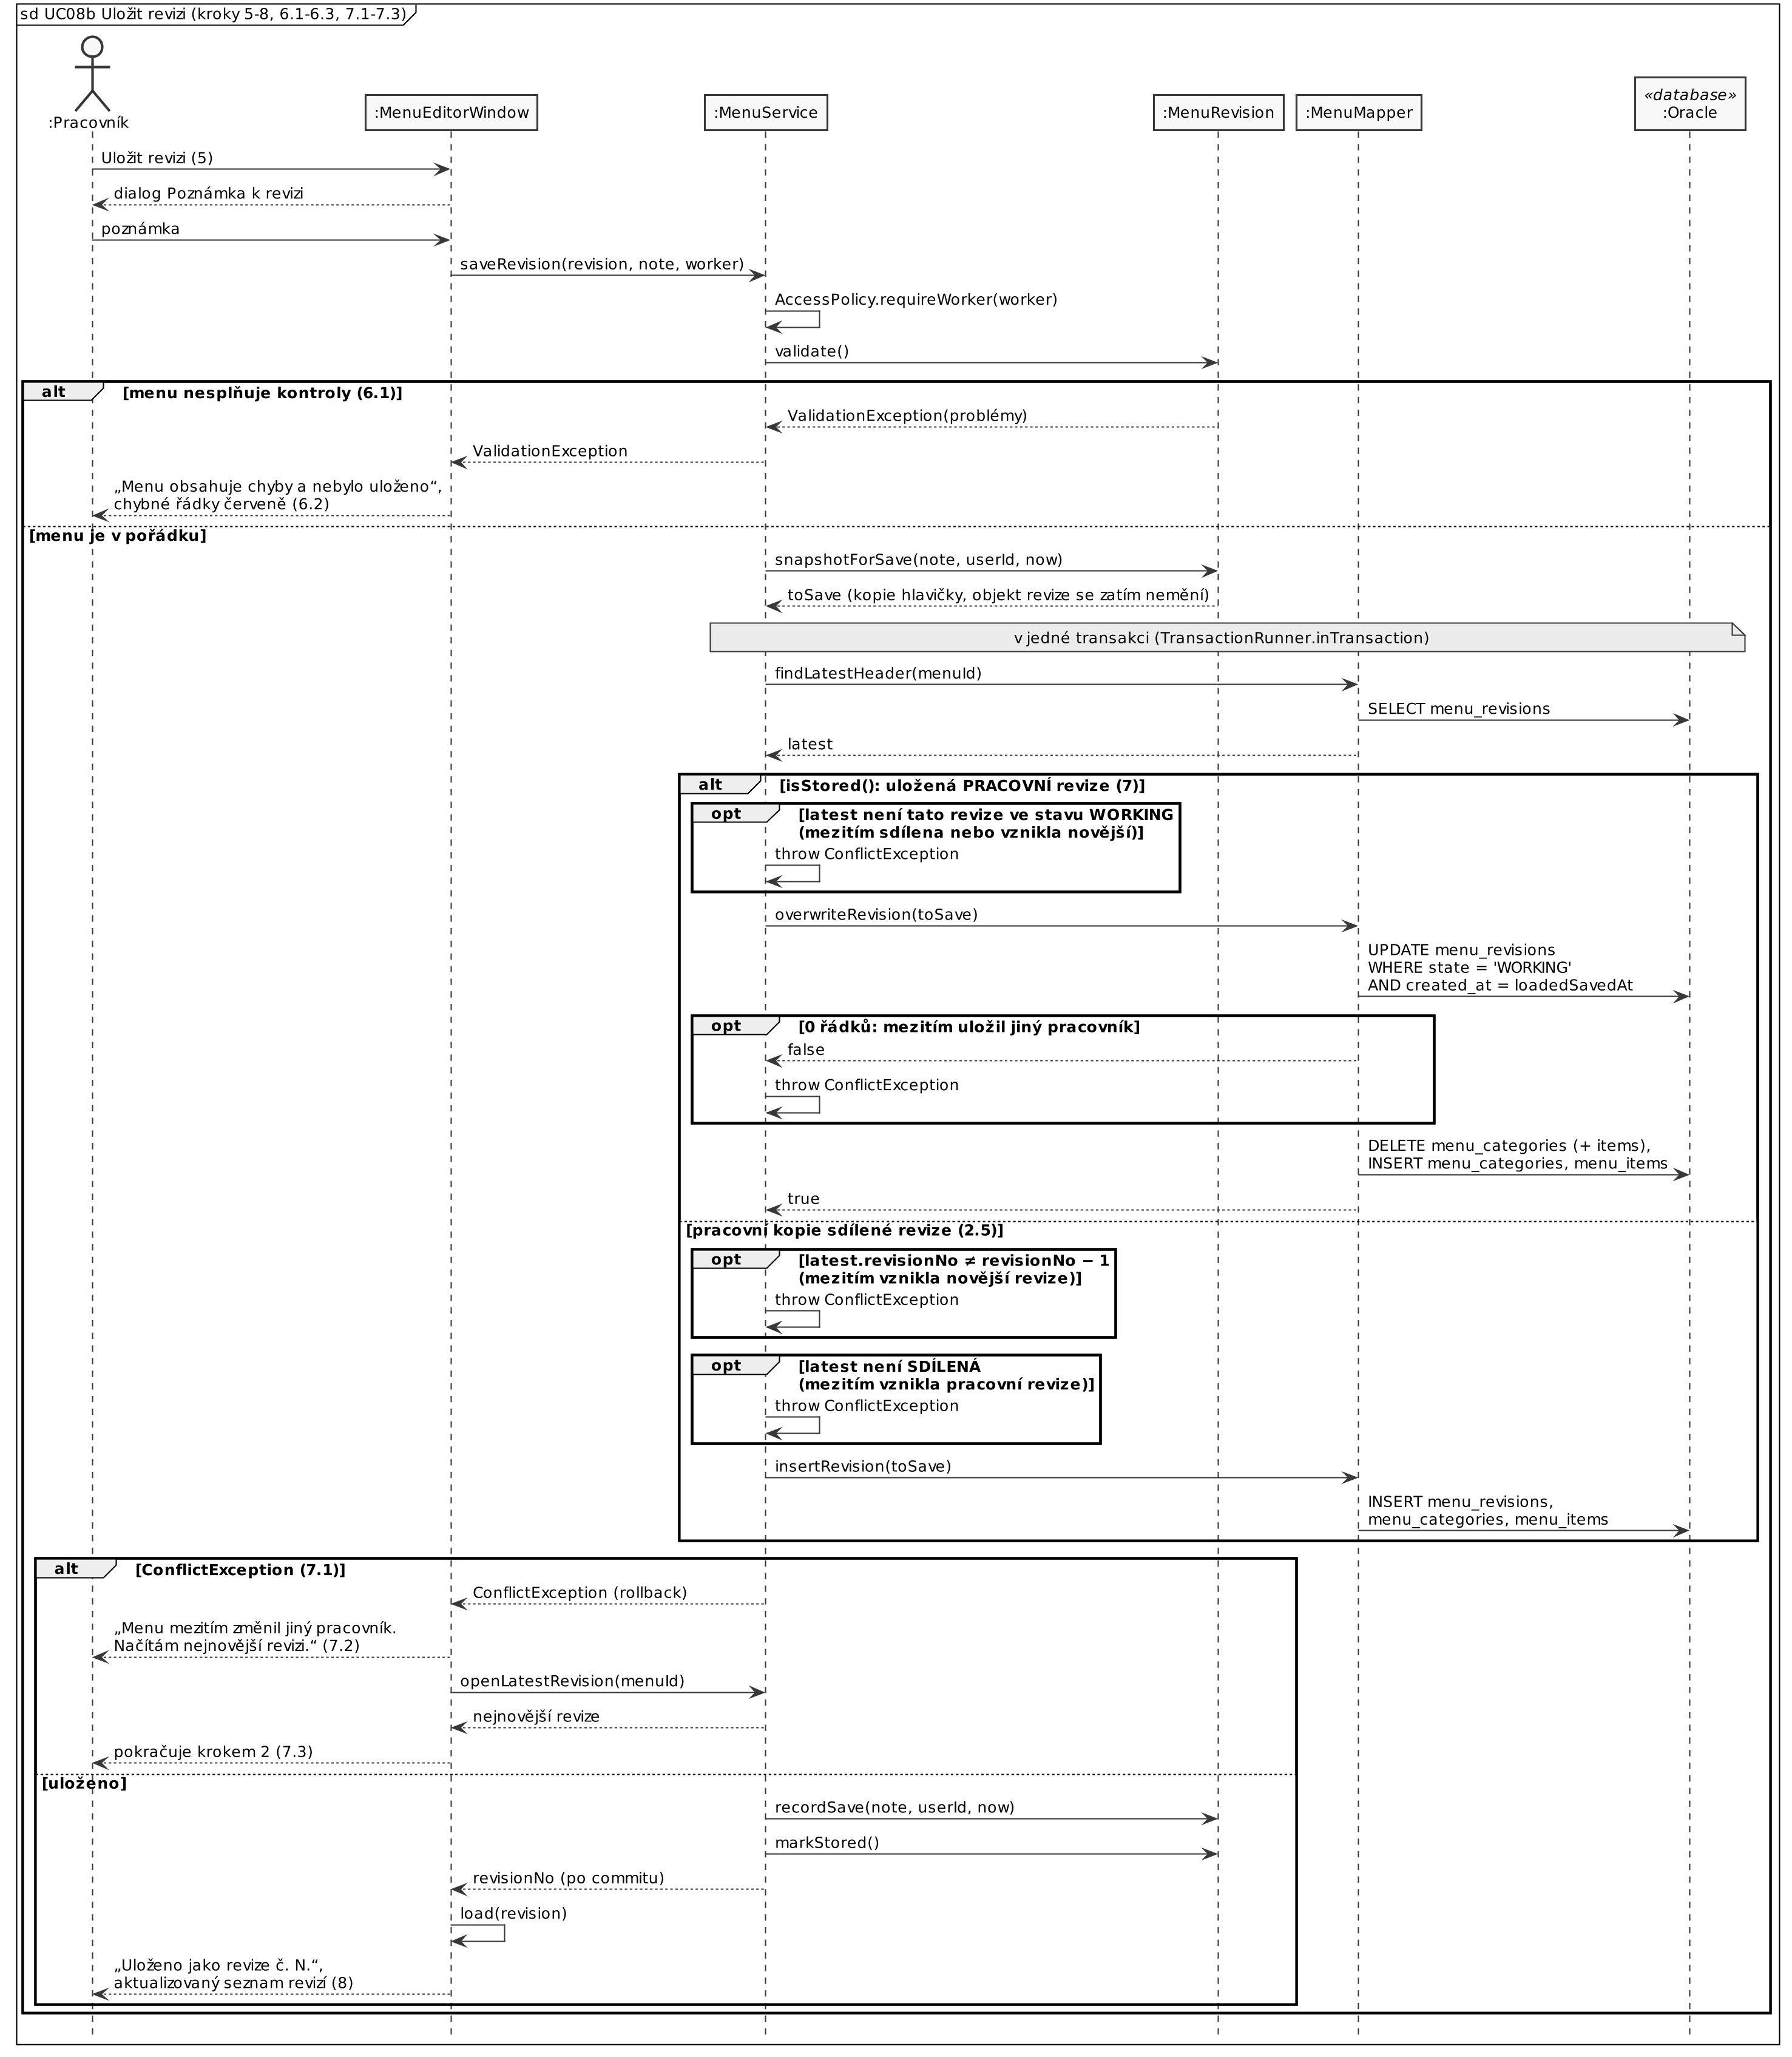
\includegraphics[width=\textwidth,height=0.85\textheight,keepaspectratio]{seq-uc08-b.png}
  \caption{Sekvenční diagram UC08 -- Uložit revizi (kroky 5--8, 6.x, 7.x)}
\end{figure}
\clearpage

\begin{figure}[H]
  \centering
  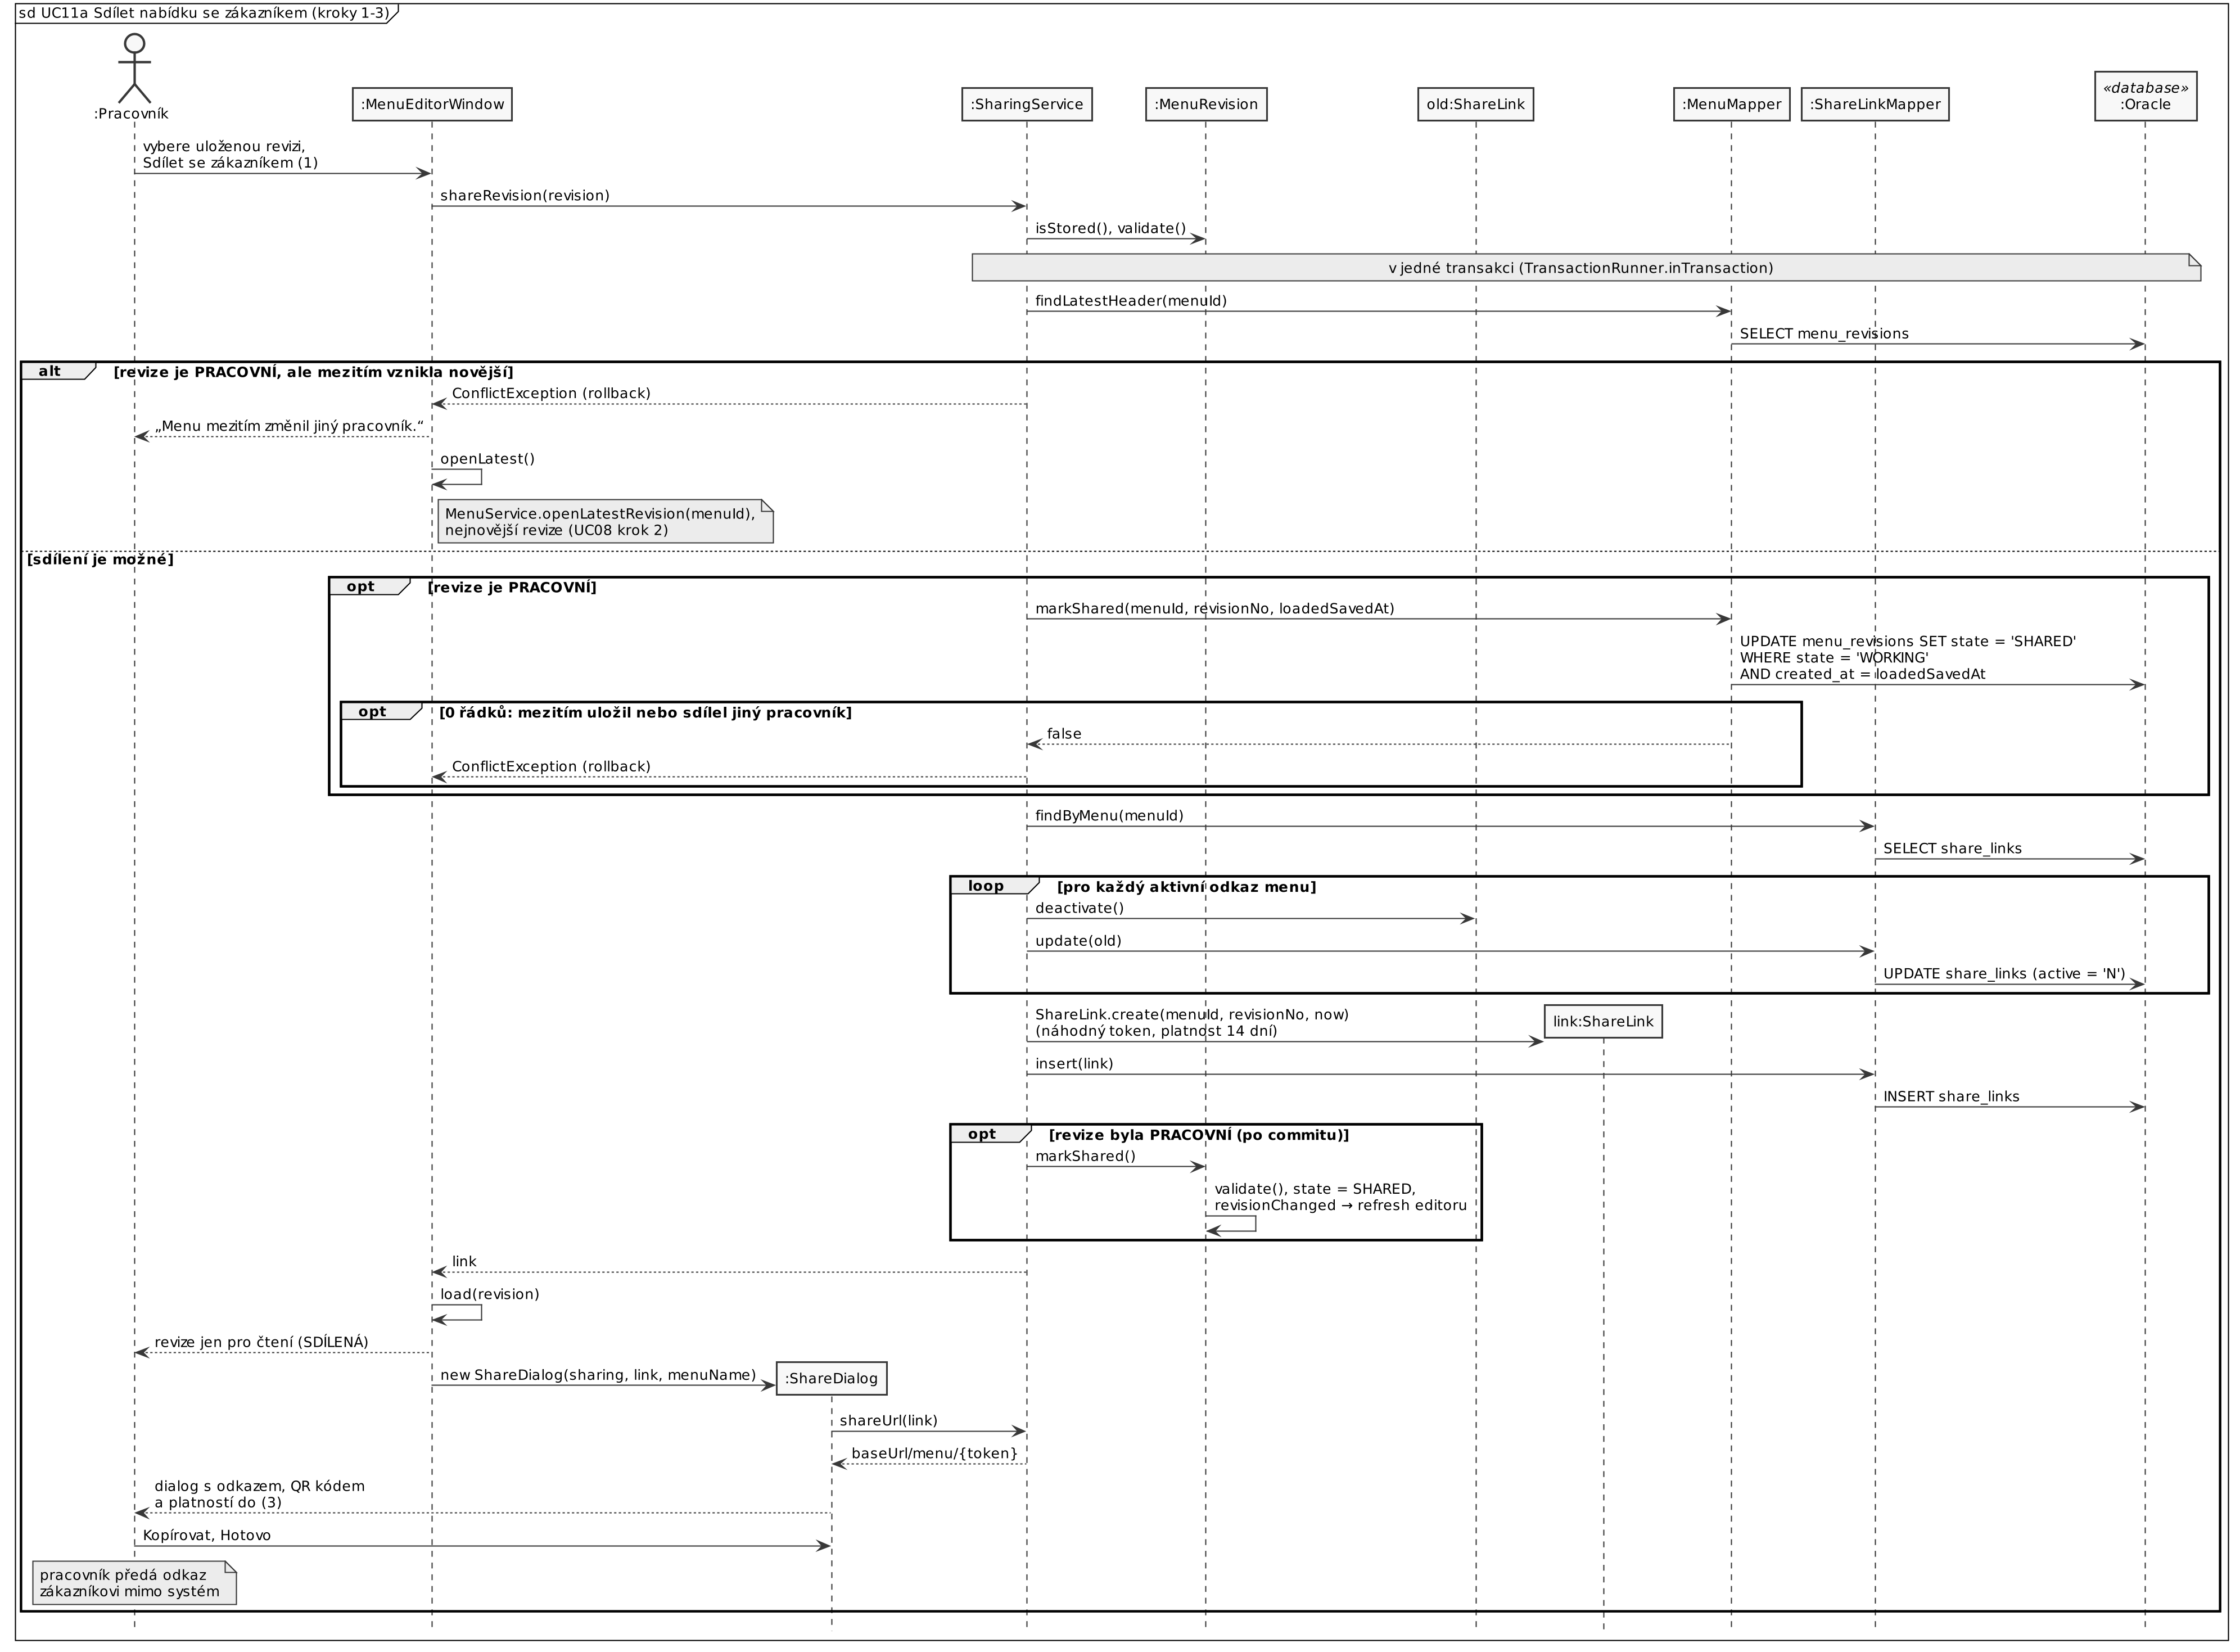
\includegraphics[width=\textwidth,height=0.85\textheight,keepaspectratio]{seq-uc11-a.png}
  \caption{Sekvenční diagram UC11 -- Sdílet nabídku (kroky 1--3)}
\end{figure}
\clearpage

\begin{figure}[H]
  \centering
  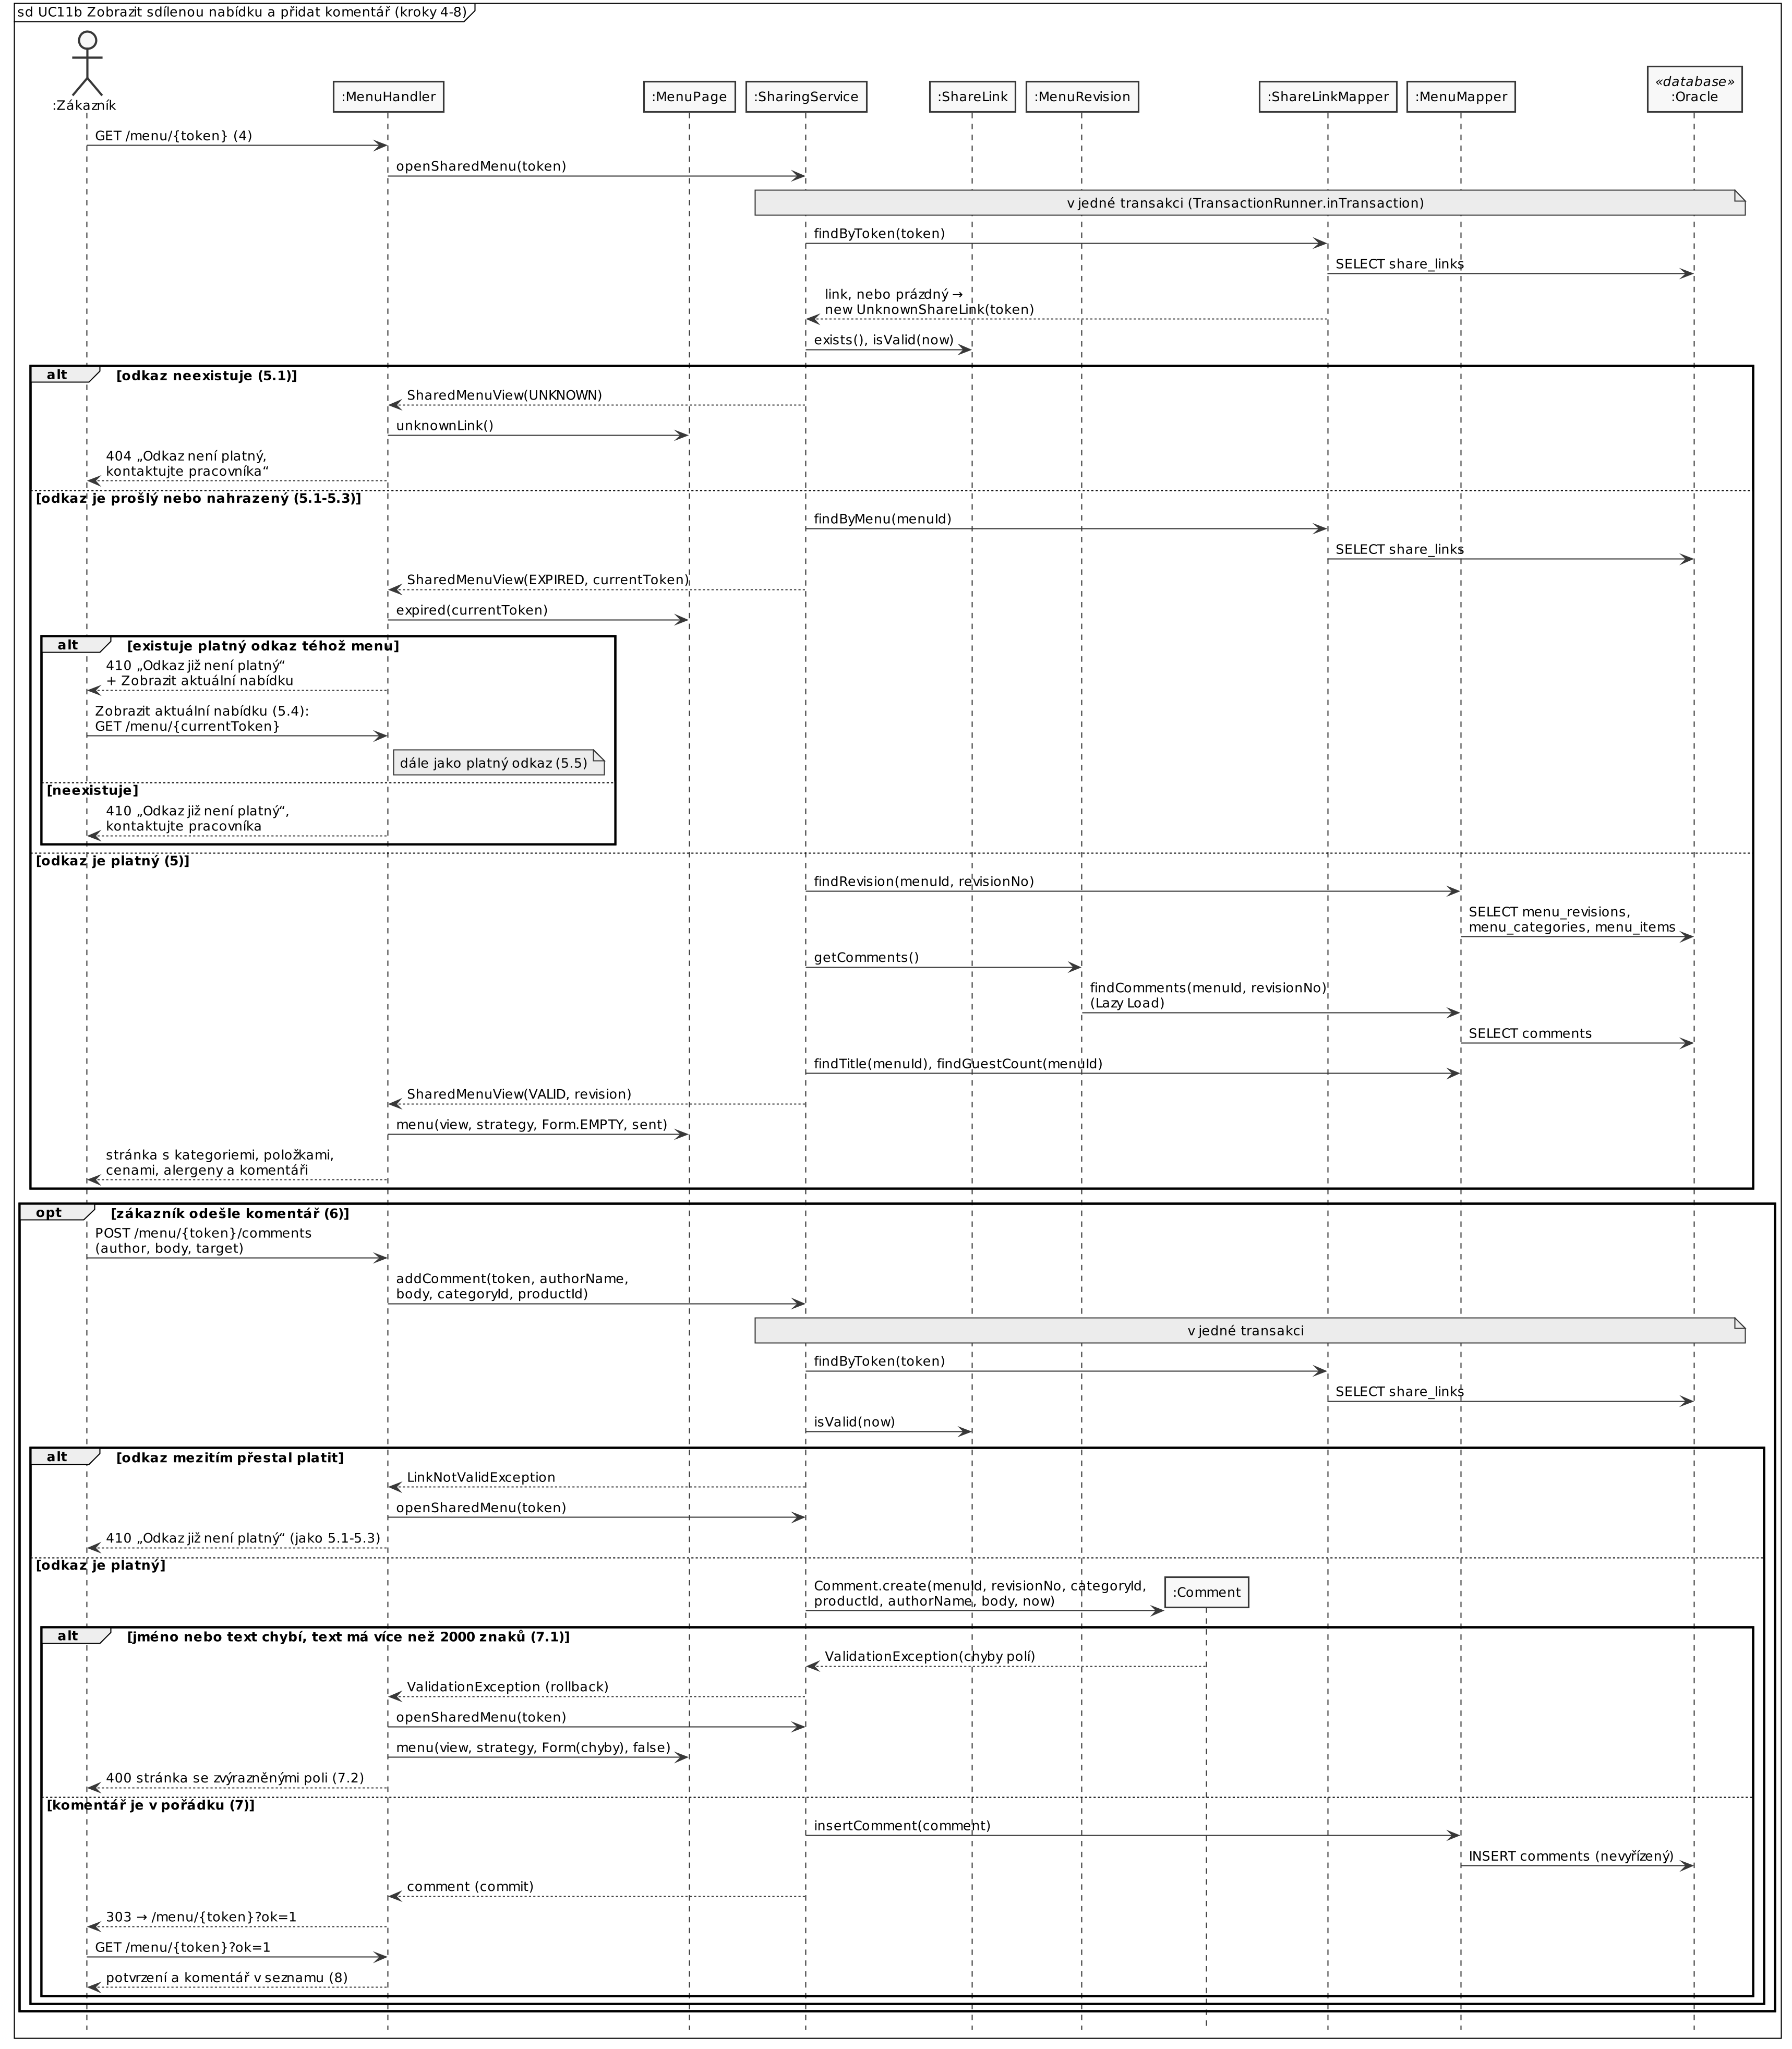
\includegraphics[width=\textwidth,height=0.85\textheight,keepaspectratio]{seq-uc11-b.png}
  \caption{Sekvenční diagram UC11 -- Web zákazníka a komentář (kroky 4--8, 5.x, 7.x)}
\end{figure}
\clearpage

\begin{figure}[H]
  \centering
  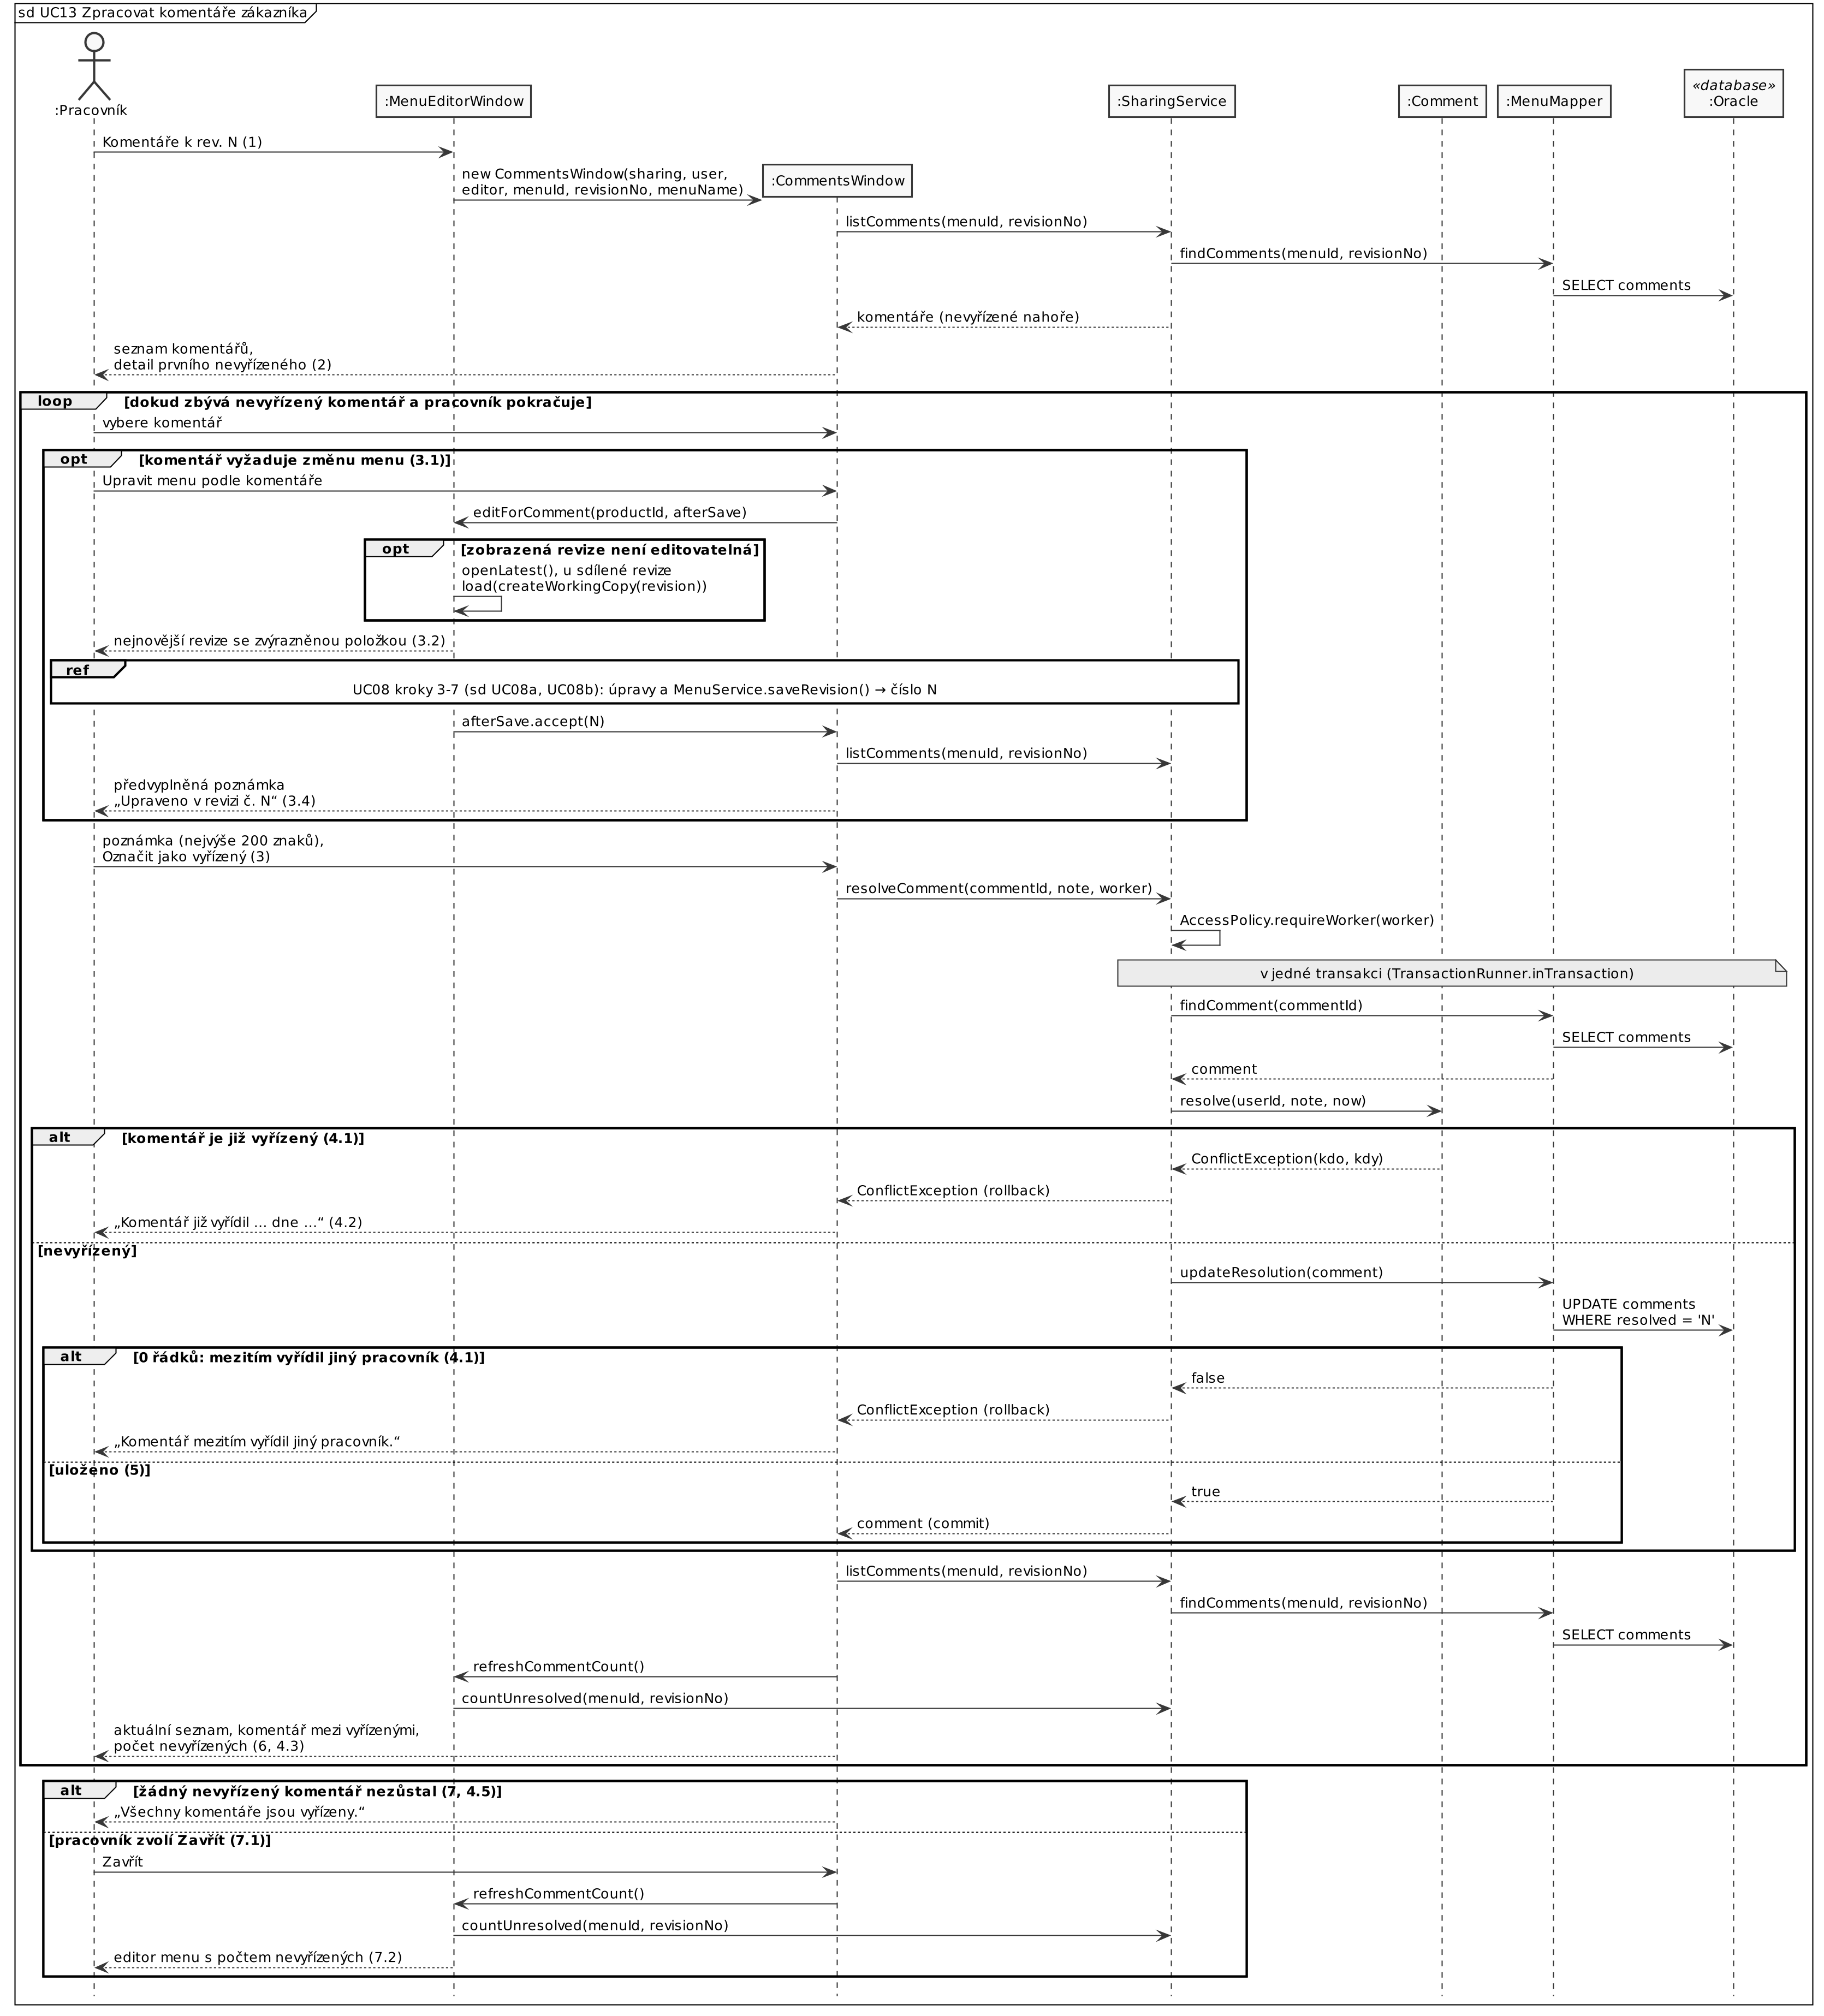
\includegraphics[width=\textwidth,height=0.85\textheight,keepaspectratio]{seq-uc13.png}
  \caption{Sekvenční diagram UC13 -- Zpracovat komentáře zákazníka}
\end{figure}
\clearpage

\begin{figure}[H]
  \centering
  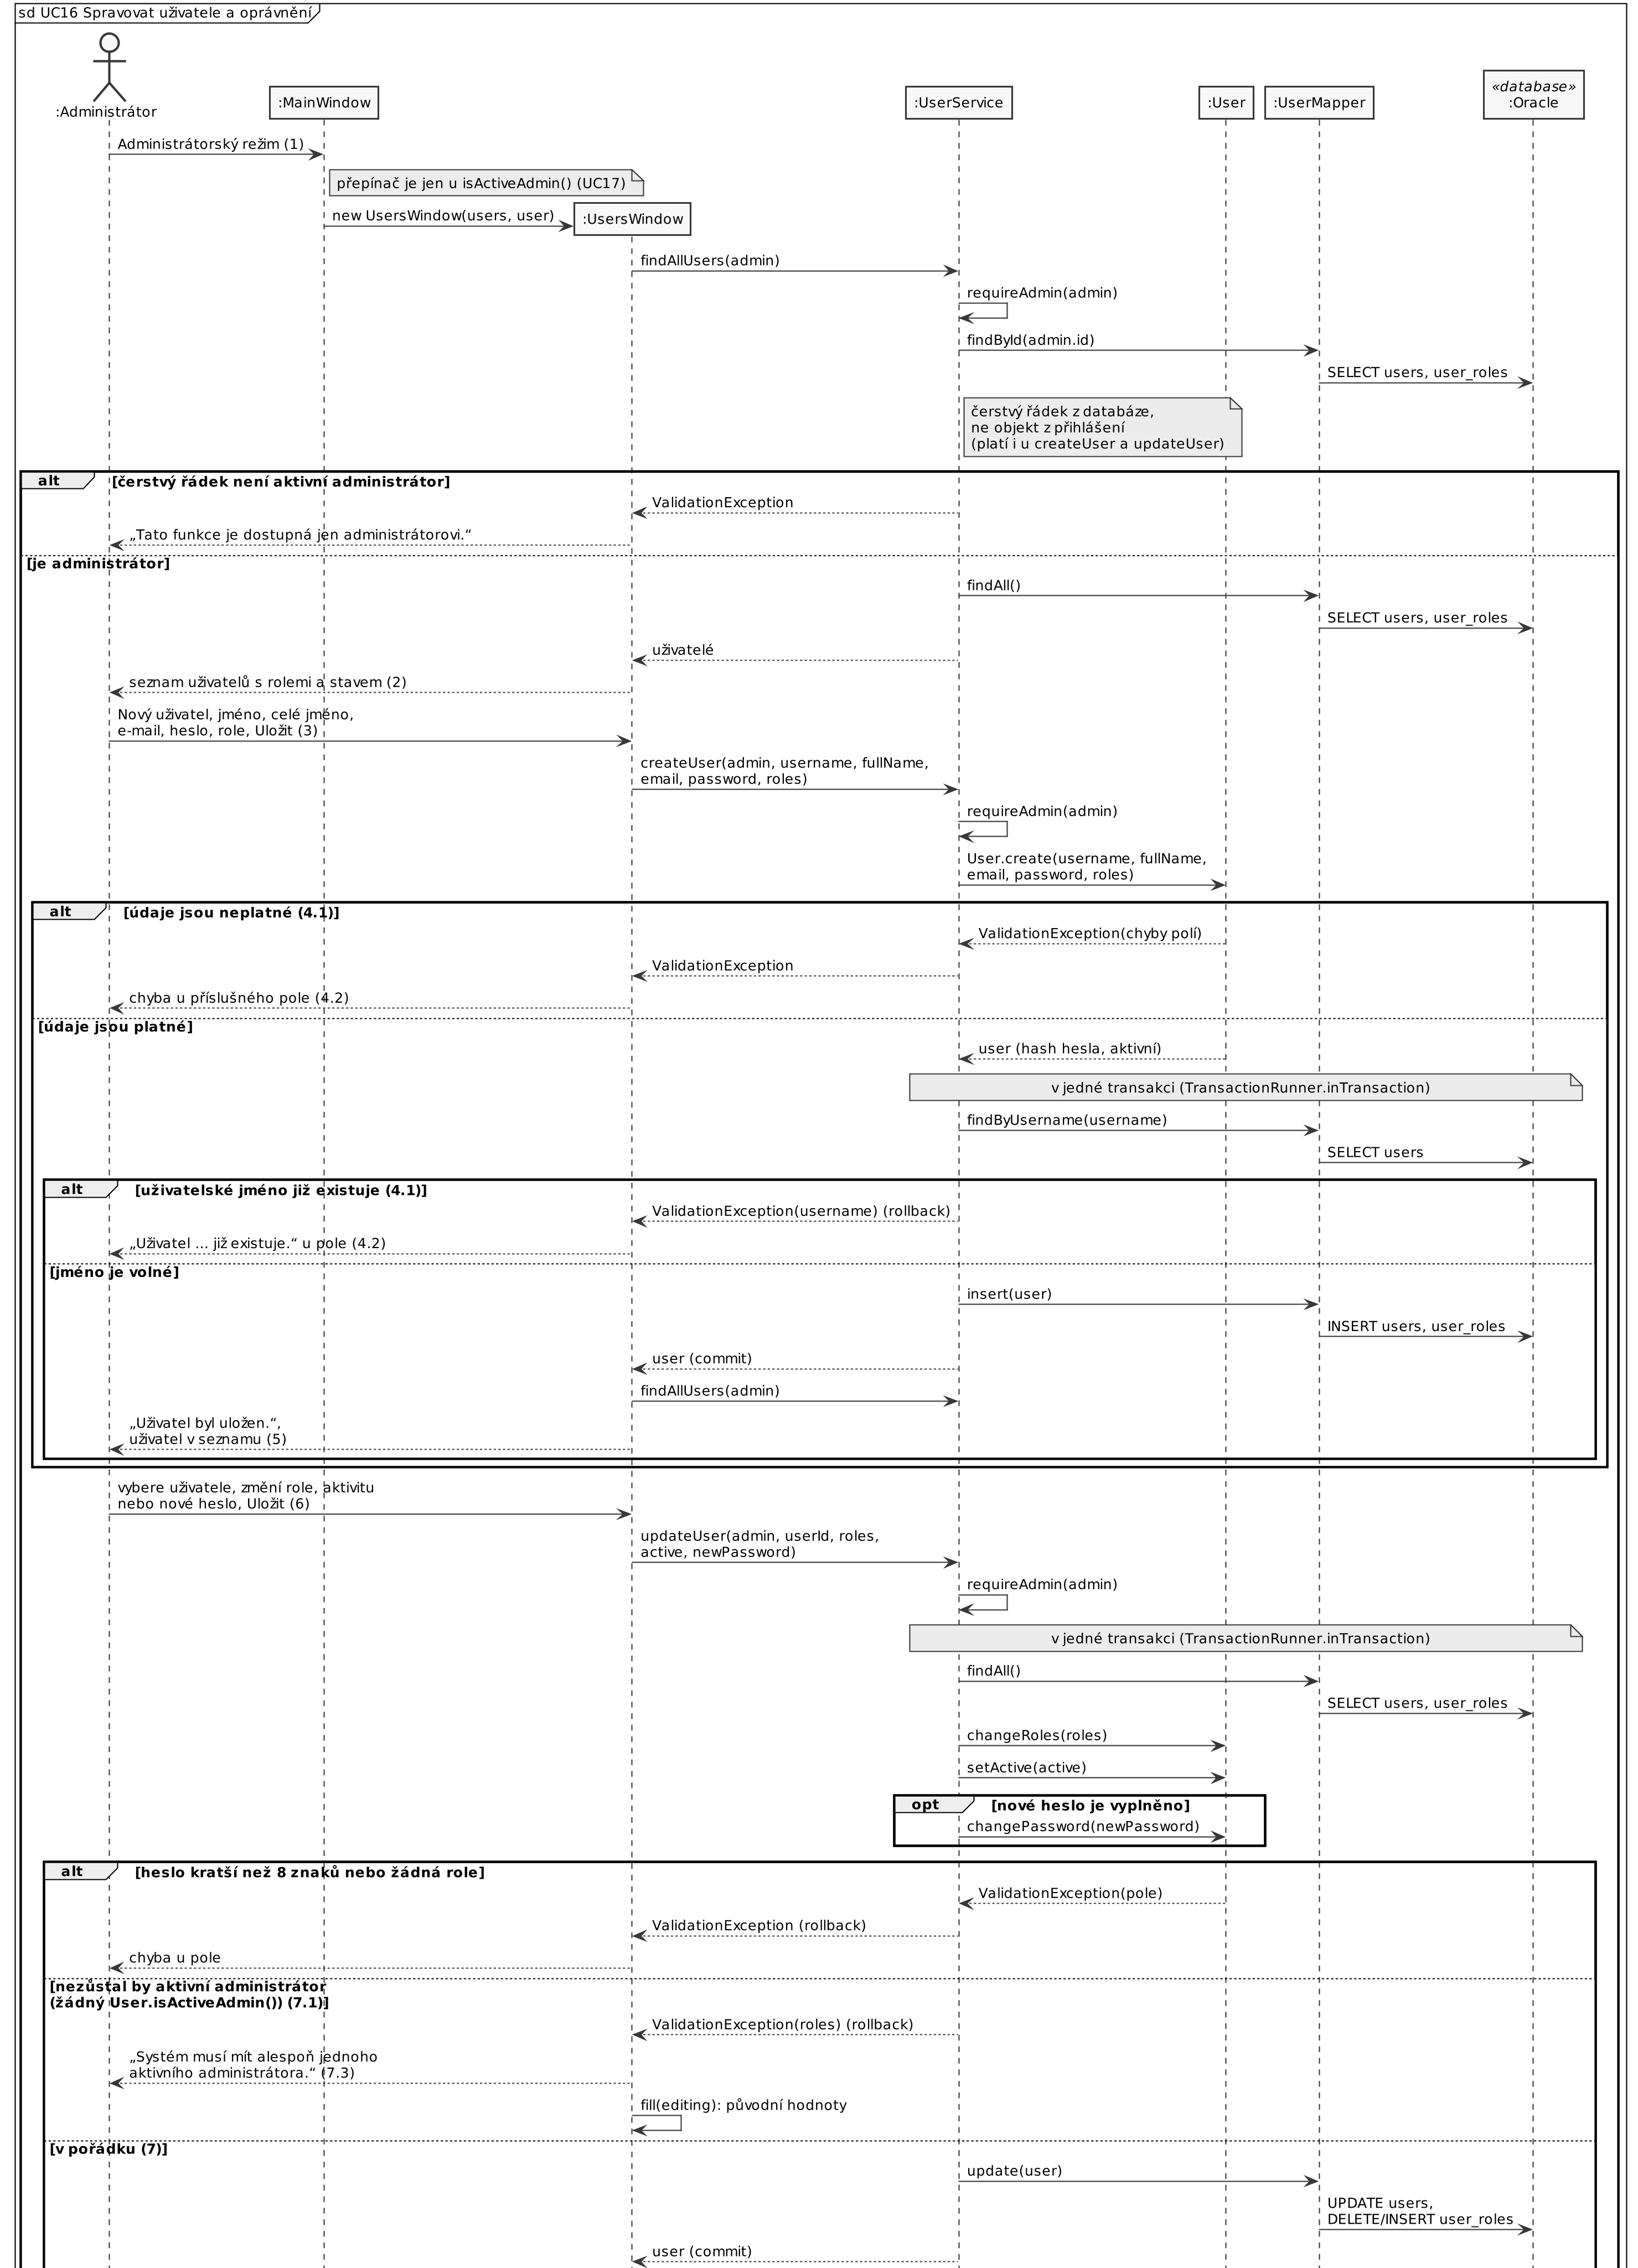
\includegraphics[width=\textwidth,height=0.85\textheight,keepaspectratio]{seq-uc16.png}
  \caption{Sekvenční diagram UC16 -- Spravovat uživatele a oprávnění}
\end{figure}
\clearpage

\subsection{Použité vzory}\label{sec:a5:vzory}

Každý vzor v této kapitole je v kódu. U vzoru je uvedená třída, která ho realizuje.

\subsubsection*{Vzory podnikových aplikací}

\begin{description}[itemsep=2pt,style=unboxed]
  \item[Layers] Aplikace má tři vrstvy v balíčcích \texttt{presentation}, \texttt{business} a \texttt{data}. Prezentační vrstva volá jen služby. Aplikační vrstva nezná datovou vrstvu, protože pracuje jen s rozhraními z \texttt{business.port}. Vrstvy propojí \texttt{AppContext}.
  \item[Domain Model] Pravidla systému jsou v doménových třídách v \texttt{business.domain}, nikoli ve službách. Například \texttt{MenuRevision} sama hlídá, zda ji lze upravit, a kontroluje obsah menu. Pravidla přístupu podle rolí jsou ve třídě \texttt{AccessPolicy} stejné vrstvy. Je to obyčejná třída s pravidly bez stavu, nepatří k žádnému z pojmenovaných vzorů.
  \item[Layer Supertype] Třída \texttt{DomainObject} je společný předek entit. Drží identifikátor a metodu \texttt{isNew}.
  \item[Value Object] \texttt{Money} je neměnná částka porovnávaná podle hodnoty. Každá operace vrací novou instanci.
  \item[Service Layer a Facade] Třídy \texttt{*Service} v \texttt{business.service} nabízejí prezentační vrstvě jednoduché operace pro kroky případů užití. Za každou operací skrývají práci s mappery, transakcí a doménovými objekty.
  \item[Data Mapper] Třídy \texttt{Oracle*Mapper} v \texttt{data.oracle} převádějí doménové objekty na řádky tabulek a zpět. Doménové objekty o databázi nic nevědí.
  \item[Identity Field] Entity drží primární klíč v \texttt{DomainObject.id}. \texttt{Jdbc.insert} ho po vložení řádku přečte z databáze a mapper ho objektu nastaví. Revize menu nemá vlastní \texttt{id} a je určena dvojicí \texttt{menuId} a \texttt{revisionNo}.
  \item[Foreign Key Mapping] Odkaz na jiný objekt je v tabulce uložený jako cizí klíč. \texttt{OracleProjectMapper} načte projekt spojením s tabulkou \texttt{customers} a sestaví objekt \texttt{Customer}. \texttt{OracleMenuMapper} stejně sestaví \texttt{Product} k položce menu.
  \item[Association Table Mapping] Vazby M:N jsou ve spojovacích tabulkách. \texttt{OracleUserMapper} ukládá role do \texttt{user\_roles} a \texttt{OracleProductMapper} alergeny do \texttt{product\_allergens}.
  \item[Dependent Mapping] Kategorie a položky menu nemají vlastní mapper. Načítá a ukládá je \texttt{OracleMenuMapper} spolu s revizí (\texttt{insertContent}). Při přepsání revize staré kategorie smaže a vloží aktuální obsah.
  \item[Single Table Inheritance] Složky, dokumenty a menu jsou v jedné tabulce \texttt{project\_nodes}. Sloupec \texttt{node\_type} určí, kterou podtřídu \texttt{ProjectNode} vytvoří \texttt{OracleProjectNodeMapper}.
  \item[Lazy Load] \texttt{OracleMenuMapper} dá revizi místo komentářů jen funkci pro jejich načtení. Komentáře se z databáze přečtou až při prvním volání \texttt{MenuRevision.getComments}. Stejně se načítá fotografie produktu (\texttt{ProductMapper.loadPhoto}).
  \item[Gateway] \texttt{DocumentStorage} je brána k druhému úložišti dokumentů a \texttt{FileDocumentStorage} ji implementuje nad adresářem souborů. Služby tak nepracují přímo se souborovým systémem.
  \item[Service Stub] \texttt{InMemoryDocumentStorage} nahrazuje skutečné úložiště v paměti. Testy služeb díky ní běží bez adresáře na disku.
  \item[Special Case] \texttt{UnknownShareLink} zastupuje token, který v databázi není. \texttt{SharingService} s ním zachází jako s běžným odkazem a nemusí kontrolovat \texttt{null}.
  \item[Kontrola souběžné změny] Uložení revize používá zjednodušenou optimistickou kontrolu ve stylu Optimistic Offline Lock. Tabulka nemá sloupec s verzí. Místo verze slouží čas posledního uložení revize. \texttt{OracleMenuMapper.overwriteRevision} přepíše revizi jen tehdy, když je ještě pracovní a čas v databázi se shoduje s časem při načtení (\texttt{getLoadedSavedAt}). Stejně se chová \texttt{markShared} při sdílení. Jinak vrátí \texttt{false} a služba vyhodí \texttt{ConflictException}. \texttt{MenuService.saveRevision} navíc ověří, že mezitím nevznikla novější revize a že pracovní kopii nepředběhla jiná pracovní revize. Objekt revize se mění až po commitu, takže neúspěšné uložení ho nezmění.
  \item[Transaction] \texttt{Database.inTransaction} spustí operaci služby v jedné transakci. Na konci provede commit a při výjimce rollback. Vnořené volání se připojí k běžící transakci.
\end{description}

\subsubsection*{Vzory GoF}

\begin{description}[itemsep=2pt,style=unboxed]
  \item[Composite] \texttt{ProjectNode} je společný typ uzlů stromu. \texttt{Folder} je složený uzel s dětmi, \texttt{Document} a \texttt{Menu} jsou listy. Například \texttt{countDocuments} a \texttt{isDeletable} se volají stejně na složku i na list.
  \item[Factory] \texttt{DataAccessFactory} vytváří všechny objekty datové vrstvy podle konfigurace. Zbytek aplikace nezná konkrétní třídy mapperů ani úložiště.
  \item[Factory Method] \texttt{NodeCreator.createIn} provede společné kroky (kontrola názvu a vložení do složky). Abstraktní metoda \texttt{createNode} nechá potomky \texttt{FolderCreator}, \texttt{MenuCreator} a \texttt{DocumentCreator} rozhodnout, jaký uzel vznikne.
  \item[Singleton] \texttt{Database} má jedinou instanci. Vytvoří ji \texttt{Database.init} při startu (volá ji \texttt{DataAccessFactory}). Mappery ji používají přes pomocnou třídu \texttt{Jdbc}, která ji získá metodou \texttt{getInstance}.
  \item[Facade] Služby v \texttt{business.service} jsou fasádou aplikační vrstvy pro desktopové okno i webový server (viz Service Layer).
  \item[Strategy] \texttt{PriceStrategy} určuje výpočet ceny řádku menu. \texttt{PriceWithoutVat} počítá cenu bez DPH a \texttt{PriceWithVat} s DPH. Uživatel strategii přepíná v editoru menu i na webu zákazníka.
  \item[Observer] \texttt{MenuRevision} je pozorovaný objekt a po každé úspěšné změně volá \texttt{MenuRevisionListener.revisionChanged}. \texttt{MenuEditorWindow} se registruje jako posluchač a obnoví tabulku a součty.
  \item[Command] Každá úprava menu je objekt s rozhraním \texttt{MenuEditCommand} (\texttt{AddCategoryCommand}, \texttt{RemoveCategoryCommand}, \texttt{AddItemCommand}, \texttt{ChangeItemCommand}, \texttt{RemoveItemCommand}). \texttt{MenuEditor} příkazy spouští, ukládá je do zásobníku a tlačítkem Zpět je vrací.
\end{description}
\endgroup
